%Les rapports ici présenté ont été écrit en langage \gls{md}, plus spécifiquement dans le dialecte nommé \foreign{Gitlab-flavored Markdown}.
%Ce dialecte supporte des éléments comme l'intégration d'images, de formules, de fragments de codes entre autres fonctionnalités.
%Ces spécificités en font un langage idéal pour écrire des rapports exploitants ces fonctionnalités et destinés à être lus au format informatique.
%De plus

\begin{nohyphen}
\section{Informations sur les rapports contenus dans la présente annexe} \label{report_infos}
Les sections suivantes contiennent les rapports intermédiaires fournis au maître de stage tout au long du \gls{project_gmsnn}.

\subsection{Format d'origine des rapports}
Le langage \gls{md}, plus spécifiquement dans le dialecte nommé \gls{git_md} (littéralement \og \gls{md} à la saveur de \gls{gitlab}\fg{}), fournit une syntaxe facile à lire et à écrire. %\foreign{Gitlab-flavored Markdown}.
Il permet la rédaction de documents agrémentés entre autres d'images, de formules, de tableaux et de fragments de codes.
Enfin, l'affichage du \gls{git_md} est supporté par \gls{gitlab}. % TODO améliorer phrase

Ces particularités en font un langage de premier choix pour l'écriture de rapports destinés à être lus au format informatique directement sur \gls{gitlab}.

\subsection{Transcription des rapports}
L'intégration des rapports intermédiaires dans ce document a nécessité l'adaptation au format papier du contenu rédigé en \gls{git_md}.

Certains éléments n'ont pas pu être transcris de façon exacte, en particulier les liens et les tableaux et images de grand taille. Ces éléments ont donc été adaptés.

\subsection{Contenu et langue des rapports}
Le contenu des rapports n'a été ni modifié ni corrigé, et est livré en anglais tel qu'écrit à l'origine.

L'anglais a été choisi comme langue de rédaction des rapports pour maintenir la cohérence avec le code, écrit et documenté en anglais lui aussi, et avec la littérature, principalement rédigée en anglais.
Ce choix évite aussi d'alourdir le contenu déjà complexe des documents avec des traductions maladroites. %TODO Je met fraiment ca ?

\end{nohyphen}

\newpage
\begin{report}{Étude des problèmes de mémoire}\label{subsec:memuse}
	% !TeX spellcheck = en_US
\section*{Analysis of memory usage}

Analysis report

by E. Marquer, 2018/05/23, Synalp and Université de Lorraine

\subsection{Abstract}

Experimental results shows (using \lstinline!nvidia-smi!) an increasing
memory usage for 4 layers, from an already enormous 3GB to more than
6GB, causing an out-of-memory error.

The objective of the following computations is to estimate the memory
consumption of the model, to confirm the hypothesis of a memory leak,
and verify that the model should not overflow memory.

\subsection{Formulas}

\subsubsection{Tensor and Variable size
estimation}

Byte size of a tensor is close to 6 times the products of all of its
dimensions. Byte size of a variable is similar to that of the
corresponding tensor.

\begin{lstlisting}[language=Python]
import torch, pickle

# Object to mesure
o = torch.autograd.Variable(torch.ones(100, 100, 100))
o = torch.ones(100, 100, 100)

len(pickle.dumps(o, 0)) / (100 * 100 * 100)
#result = 6
\end{lstlisting}

\subsubsection{Computations}
\vspace{-2em}
\begin{equation}
\begin{aligned}
total 
&= hidden\_states + msnn\_weights + emb\_weights + out\_weights \\\\
&= detach\_interval * (growth\_factor + 1) * layers * 6 * (hidden\_size * batch\_size * sequence\_length) \\
& + (((layer - 1) * 8 * hidden\_size * (hidden\_size + 1)) \\
& + 4 * hidden\_size * (hidden\_size + emb\_size + 2)) * 6  \\
& + (nwords * (emb\_size + 1)) * 6 \\
& + (nwords * (layers * hidden\_size)) * 6 \\\\
&= 6 * (detach\_interval * (growth\_factor + 1) * layers * 
(hidden\_size * batch\_size * sequence\_length) \\
& + ((layers - 1) * 8 * hidden\_size * (hidden\_size + 1)) \\
& + 4 * hidden\_size * (hidden\_size + emb\_size + 2)  \\
& + (nwords * (emb\_size + 1)) \\
& + (nwords * (layers * hidden\_size)))
\end{aligned}
\end{equation}

\begin{equation}
\begin{aligned}
hidden\_states &= total\_history * 6 * dim \\
               &= detach\_interval * (growth\_factor + 1) * layers * 6 * dim \\
               &= detach\_interval * (growth\_factor + 1) * layers * 6 * \\
               & (hidden\_size * batch\_size * sequence\_length)
\end{aligned}
\end{equation}

\begin{equation}
\begin{aligned}
msnn\_layer\_weights &= weights\_ih + weights\_hh + bias\_ih + bias\_hh \\
                     &= 4 * hidden\_size * input\_size + 4 * hidden\_size * hidden\_size \\
                     & + 4 * hidden\_size + 4 * hidden\_size \\
                     &= 4 * hidden\_size * (hidden\_size + input\_size + 2) \\
                     &= \begin{cases}
                        8 * hidden\_size * (hidden\_size + 1) &\text{for all layers exept the first one} \\
                        4 * hidden\_size * (hidden\_size + emb\_size + 2)  &\text{for the first layer}
                        \end{cases}
\end{aligned}
\end{equation}

\begin{equation}
\begin{aligned}
msnn\_weights &= msnn\_layer\_weights * layers \\
              &= ((layers - 1) * 8 * hidden\_size * (hidden\_size + 1))\\
              & + 4 * hidden\_size * (hidden\_size + emb\_size + 2)
\end{aligned}
\end{equation}

\begin{equation}
\begin{aligned}
emb\_weights &= (bias + weights) * 6 \\
            &= (nwords * emb\_size + emb\_size))* 6 \\
            &= (nwords * (emb\_size + 1)) * 6
\end{aligned}
\end{equation}

\begin{equation}
out\_weights = (nwords * (layers * hidden\_size)) * 6
\end{equation}

\newpage
\subsubsection{Estimate with basic set of parameters}

\begin{lstlisting}[language=Python]
detach_interval = 50
growth_factor = 5
layers = 7
hidden_size = 1840 / 4
batch_size = 2
sequence_length = 100
emb_size = 400
nwords = 205

total = 6 * (detach_interval * (growth_factor + 1) * layers * hidden_size * batch_size * sequence_length + ((layers - 1) * 8 * hidden_size * (hidden_size + 1)) + 4 * hidden_size * (hidden_size + emb_size + 2) + (nwords * (emb_size + 1)) + (nwords * (layers * hidden_size)))

"{}GB {}MB {}kB {}B".format(int(total%(1024**4) / 1024**3), int(total%(1024**3) / 1024**2), int(total%(1024**2) / 1024), int(total%1024))
# result: '1GB 741MB 614kB 9B'
\end{lstlisting}

\newpage
\rotatebox{90}{
\begin{tabular}{|cccccccc|r|}
\hline
detach\_interval & growth\_factor & layers & hidden\_size & batch\_size & sequence\_length & emb\_size & nwords & total\\
\hline
50 & 5 & 7 & 1840 / 4 & 2 & 200 / batch\_size & 400 & 205 & 1GB 153MB 68kB 6B\\
\textbf{100} & 5 & 7 & 1840 / 4 & 2 & 200 / batch\_size & 400 & 205 & 2GB 234MB 579kB 262B\\
\textbf{200} & 5 & 7 & 1840 / 4 & 2 & 200 / batch\_size & 400 & 205 & 4GB 397MB 577kB 774B\\
50 & \textbf{10} & 7 & 1840 / 4 & 2 & 200 / batch\_size & 400 & 205 & 2GB 50MB 323kB 390B\\
50 & 5 & \textbf{6} & 1840 / 4 & 2 & 200 / batch\_size & 400 & 205 & 1008MB 912kB 414B\\
50 & 5 & \textbf{5} & 1840 / 4 & 2 & 200 / batch\_size & 400 & 205 & 840MB 732kB 822B\\
50 & 5 & \textbf{4} & 1840 / 4 & 2 & 200 / batch\_size & 400 & 205 & 672MB 553kB 206B\\
50 & 5 & \textbf{3} & 1840 / 4 & 2 & 200 / batch\_size & 400 & 205 & 504MB 373kB 614B\\
50 & 5 & \textbf{2} & 1840 / 4 & 2 & 200 / batch\_size & 400 & 205 & 336MB 193kB 1022B\\
50 & 5 & \textbf{1} & 1840 / 4 & 2 & 200 / batch\_size & 400 & 205 & 168MB 14kB 406B\\
50 & 5 & 7 & \textbf{1840 / 2} & 2 & 200 / batch\_size & 400 & 205 & 2GB 431MB 598kB 94B\\
50 & 5 & 7 & \textbf{1840 / 8} & 2 & 200 / batch\_size & 400 & 205 & 573MB 28kB 890B\\
50 & 5 & 7 & 1840 / 4 & \textbf{1} & \textbf{200 / batch\_size} & 400 & 205 & 1GB 153MB 68kB 6B\\
50 & 5 & 7 & 1840 / 4 & 2 & \textbf{200} & 400 & 205 & 2GB 234MB 579kB 262B\\
50 & 5 & 7 & 1840 / 4 & 2 & 200 / batch\_size & \textbf{200} & 205 & 1GB 150MB 743kB 534B\\
50 & 5 & 7 & 1840 / 4 & 2 & 200 / batch\_size & \textbf{800} & 205 & 1GB 157MB 764kB 998B\\
50 & 5 & 7 & 1840 / 4 & 2 & 200 / batch\_size & 400 & \textbf{500} & 1GB 159MB 182kB 984B\\
\hline
\end{tabular}
}

\newpage
\paragraph{Most impactful factors
(memory-wise)}

\begin{itemize}
\item
  \lstinline!detach_interval!: \lstinline!detach_interval * 2! =
  \lstinline!memory * 2!
\item
  \lstinline!growth_factor!: \lstinline!growth_factor * 2! =
  \lstinline!memory * 2!
\item
  \lstinline!hidden_size!: \lstinline!hidden_size * 2! =
  \lstinline!memory * 2!
\item
  \lstinline!batch_size * sequence_length! (number of examples by
  sequence): \lstinline!batch_size*sequence_length * 2! =
  \lstinline!memory * 2!
\item
  \lstinline!layers!: \lstinline!layers * 2! = \lstinline!layers * 2!
\end{itemize}

The others factors considered (emb\_size and nwords) have almost no
impact on memory. It confirms that the most memoryphage element is the
MSNN. Also, to keep a stable memory usage,
\lstinline!batch_size * sequence_length! ratio must be kept constant;
increasing \lstinline!batch_size! while lowering
\lstinline!sequence_length! can increase processing speed whithout
impacting memory usage.

\subparagraph{Impact of layer increase}
\subparagraph*{}\vspace{-2em}{We can notice that the impacts of layers is most noticeable during the
first phases of training, during the creation of the first layer. Later
on, the creation frequency of new layers is small, and the change is
minimal. For example, from 6 to 7 layer, we need \(`12500`\) sequences
to pass, and the increase of memory of about \(`7/6`\); from 7 to 8
layer, we need \(`62500`\) sequences to pass, and the increase of memory
of about \(`8/7`\); from 8 to 9 layer, we need \(`312500`\) sequences to
pass, and the increase of memory of about \(`9/8`\); and so on.}

\subsubsection{Partial derivatives:}

\begin{lstlisting}
d = detach_interval
g = growth_factor
l = layers
h = hidden_size
b = batch_size
s = sequence_length
e = emb_size
n = nwords

complete formula:
6 * (
	d * (g + 1) * l * h * b * s +
	((l - 1) * 8 * h * (h + 1)) +
	4 * h * (h + e + 2) +
	(n * (e + 1)) +
	(n * (l * h))
)

simplified formula:
6*(8*l*h^2 + l*d*g*h*b*s + l*d*h*b*s + 8*l*h + l*n*h + 4*e*h + e*n + n - 4*h^2)

partial derivates on given variable:
d: (6(8*l*h^2 - 4*h^2 + l*d*g*h*b*s + l*d*h*b*s + 8*l*h + 4*e*h + l*n*h + e*n + n))
g: 6*l*d*h*b*s
l: 6*(d*h*b*s*(g+1) + 8*h*(h+1) + nh)
h: 6*(l*d*g*b*s + l*d*b*s + l*n + 16*l*h + 8*l + 4*e - 8*h)
b: 6*l*d*h*s*(g+1)
s: 6*l*d*h*b*(g+1)
e: 0
n: 6*(l*h+e+1)
\end{lstlisting}


\end{report}
\begin{report}{Sauvegarde du modèle}\label{subsec:save}
	\section*{Analysis and implementation of job save and
restart}

Implementation report

by E. Marquer, 2018/05/24\\
Synalp and Université de Lorraine

\subsection{Abstract}

As the jobs are taking longer than an hour per epoch, it has become
necessary to keep an image of the model, the training parameters and the
current state of the model to be able to interrupt training when needed.

Multiple choices are available:
\begin{itemize}
\item an easy but heavy serialisation (pickle) of the whole system;
\item a ``full'' save of the model and parameters, excluding everything that can be recomputed easily;
\item a ``partial'' save of the model, removing a part of the less important
information.
\end{itemize}

\subsection{\texorpdfstring{\textbf{End solution: saving using pytorch
utilities}}{End solution: saving using pytorch utilities}}

The saving solution currently implemented is the
\lstinline!torch.save(trainer, file)! and
\lstinline!trainer = torch.load(file)! and the alternatie version
\lstinline!trainer = torch.load(file, map_location=lambda storage, loc: storage)!
allowing the loading of a CUDA model out of CUDA.

This solution posed a number of problems when it was first tested
(internal non-parameter atributes where not correctly saved and loaded),
that is why it was not considered at first.

But a more recent try resulted in a perfect result, replacing the need
of a custom serialisation system.

\subsection{Full serialisation}

This kind of serialisation is done thanks the \lstinline!pickle!
package, on the whole Trainer object.

\begin{lstlisting}[language=Python]
import pickle

def load(filename: str) -> object:
    with open(filename, 'rb') as f:
        return pickle.load(f)

def save(filename: str, trainer: object) -> None:
    with open(filename, 'wb') as f:
        pickle.dump(trainer, f)
\end{lstlisting}

\subsection{Full save}

\subsubsection{Elements to save}

\begin{itemize}
\item
  Corpus file name
\item
  \lstinline!cuda_on!
\item
  \lstinline!batch_size!
\item
  Trainer

  \begin{itemize}
  \item
    Model (see specific points)
  \item
    \lstinline!self.epoch! current epoch
  \item
    \lstinline!self.batch! and \lstinline!self.i! current position in
    training epoch
  \item
    \lstinline!self.start_time! needs a litle work: storing the elapsed
    time, and when loading, remove elapsed time from load time
  \item
    \lstinline!self.log_interval!
  \item
    \lstinline!self.save_interval!
  \item
    \lstinline!self.bptt!
  \item
    \lstinline!self.nwords!
  \item
    \lstinline!self.repackage_interval!
  \item
    \lstinline!self.repackage_strategy!
  \item
    \lstinline!self.reset_growth!
  \item
    \lstinline!self.reset_hidden!
  \item
    \lstinline!self.epochs!
  \item
    \lstinline!self.save_folder!
  \end{itemize}
\item
  Model (MSNN)

  \begin{itemize}
  \item
    \lstinline!self.training!
  \item
    input layer (embeddings) using \lstinline!torch.save(self.emb, f)!
    and \lstinline!torch.load(f)!
  \item
    MSNN (see specific points)
  \item
    output layer (linear)
  \end{itemize}
\item
  MSNN

  \begin{itemize}
  \item
    Final

    \begin{itemize}
    \item
      \lstinline!self.input_size!
    \item
      \lstinline!self.hidden_size!
    \item
      \lstinline!self.growth_factor!
    \item
      \lstinline!self.batch_size!
    \item
      \lstinline!self.cuda_on!
    \item
      \lstinline!self.layer_id!
    \item
      \lstinline!self.max_detach!
    \item
      \lstinline!self.repackage_strategy!
    \item
      \lstinline!self.max_layers!
    \end{itemize}
  \item
    Next MSNN
  \item
    \lstinline!self.detach_count!
  \item
    \lstinline!self.rnn!
  \item
    \lstinline!self.hidden!
  \item
    \lstinline!self.seq_count!
  \item
    \lstinline!self.detach_count!
  \item
    \lstinline!self.transmitted_output!
  \item
    \lstinline!self.transmitted_hidden!
  \end{itemize}
\end{itemize}

\subsubsection{Elements to forget and
recreate}

\begin{itemize}
\item
  Trainer

  \begin{itemize}
  \item
    Corpus

    \begin{itemize}
    \item
      Corpus file name is needed
    \end{itemize}
  \item
    Optimizer: reasign learning rate, weight\_decay and model's
    parameters (create after model is loaded) using
    \lstinline!torch.optim.SGD(model.parameters(), lr=args.lr, weight_decay=args.weight_decay)!
  \item
    Criterion: \lstinline!criterion = torch.nn.CrossEntropyLoss()!
  \item
    \lstinline!self.layers! using
    \lstinline!self.model.msnn.get_layers()! (create after model is
    loaded)
  \item
    \lstinline!self.train_data! using
    \lstinline!batchify(corpus.train, batch_size, cuda_on)!
  \item
    \lstinline!self.val_data! using
    \lstinline!batchify(corpus.valid, batch_size, cuda_on)!
  \item
    \lstinline!self.plotdata! using
    \lstinline!{"Epoch": None, "Layer": None, "Frac": None}! and
    \lstinline!self.init_plotter()! (perhaps with a new file, otherwise
    in append mode without cleaning the file)
  \item
    \lstinline!self.msnn_backup!, sould be empty if the new backup
    system (using the \lstinline!with! statement) is implemented
  \end{itemize}
\item
  Model

  \begin{itemize}
  \item
    None
  \end{itemize}
\item
  MSNN

  \begin{itemize}
  \item
    \lstinline!self.tensors!
  \end{itemize}
\end{itemize}

\subsection{Partial save}

The elements to keep are the same as with the Full save, except: -
hidden states and transmitted output are to be detached

\subsection{Other things that need to be added to interrupt and resume
job}

\subsubsection{Methods to interrupt and resume epoch loop and training
loop}

\paragraph{Interruption strategy}

Interruption can be done by:
\begin{itemize}
\item saving the state at specific timestep;
\item saving automatically when shutting down.
\end{itemize}

The second option isn't realy realistic, as an interuption wouldn't
allow a big enough margin to save the model. Even thought, it could be
added to allow manual interruption at certain timesteps (smaller than
the ones implemented in the first option).

As the first option is the only viable one, multiple timesteps are
possible, from the shortest to the longest:
\begin{itemize}
\item after each operation (example: after forward pass, and after backward pass, and after optimization \ldots{});
\item after each sequence;
\item after \emph{n} sequences;
\item  after each epoch;
\item  after \emph{n} epochs;
\item  after the whole training.
\end{itemize}

Option {[}1.{]} is not viable, as it would consume a lot of time
relative to each computation for the sole writing process. Option
{[}3.{]}, of which option {[}2.{]} is a specific case, allows both a
fine granulation with only a minimal loss if anything were to occur, and
a reduced burden computation-wise. From option {[}4.{]} onward, the save
time is negligible, and even if the granulation is mediocre, it offers
fine milestones for specific usage (usage of an already trained mode for
example).

Currently, at creation time, with no history, the model save file is
about 770MB.

What will be implemented is thoe third option, saving the model after
\emph{n} sequences.

\paragraph{Resume strategy}\label{resume-strategy}

It will be necessary to adapt the training loodps a little to allow
resuming at any sequence in any epoch.

\subsection{Other methods implemented}\label{other-methods-implemented}

\subsubsection{\texorpdfstring{Method using \texttt{with} keyword for
backup system, during
evaluation}{Method using with keyword for backup system, during evaluation}}\label{method-using-with-keyword-for-backup-system-during-evaluation}

\begin{lstlisting}[language=Python]
class BackupContextManager:
    def __init__(self, model: DetRNN):
        self.model = model
        
    def __enter__(self):
        # Backing up training linked data
        self.msnn_backup = self.model.msnn.backup()

    def __exit__(self, type, value, traceback):
        # Restoring training linked data
        self.model.msnn.restore(self.msnn_backup)


with BackupContextManager(model):
    """Do computations"""
\end{lstlisting}


\end{report}
\begin{report}{Tentative de solution pour les fuites mémoires}\label{subsec:memleak}\label{subsec:hist}
	% !TeX spellcheck = en_US
\section*{Analysis of a source of the memory leak problem: the history
management
system}

Analysis report

by E. Marquer, 2018/05/28, Synalp and Université de Lorraine

\subsection{Abstract}

A big memory leak is present in the model. One of the identified cause
is a malfunction in the history management system.

\subsection{Problem}

It seems simply detaching a hidden state is not enough:

With a graph:
\begin{lstlisting}
                        3.1 --------------------------- 3.2 -->
                         |                               |
        2.1 ----------- 2.2 ----------- 2.3 ----------- 2.4 -->
         |               |               |               |
1.1 --- 1.2 --- 1.3 --- 1.4 --- 1.5 --- 1.6 --- 1.7 --- 1.8 -->
\end{lstlisting}
where all nodes are hidden states, and each layer is a line, with a
transmission rate of 1 transmission every 2 hidden state.

When detaching every 2 hidden, with \lstinline![i.j]! a detached node,
the graph becomes:

\begin{lstlisting}
                        3.1 --------------------------- 3.2 -->
                         |                               |
        2.1 ----------- 2.2            [2.3]----------- 2.4 -->
         |               |                               |
1.1 --- 1.2    [1.3]--- 1.4    [1.5]--- 1.6    [1.7]--- 1.8 -->
\end{lstlisting}

But it should be:

\begin{lstlisting}
                        3.1 --------------------------- 3.2 -->
                         |                               |
        2.1 ----------- 2.2            [2.3]----------- 2.4 -->
                                                         |
1.1     1.2    [1.3]    1.4    [1.5]--- 1.6    [1.7]--- 1.8 -->
\end{lstlisting}

Or with a more aggressive strategy:

\newpage
\begin{lstlisting}
                        3.1 --------------------------- 3.2 -->
                                                         |
        2.1             2.2            [2.3]----------- 2.4 -->
                                                         |
1.1     1.2    [1.3]    1.4    [1.5]    1.6    [1.7]--- 1.8 -->
\end{lstlisting}

\subsection{Solution}

To solve the problem, keeping track of all history is necessary, and
with the way PyTorch works, it won't be a problem to keep references to
history before deleting them

\end{report}
\begin{report}{Problèmes théoriques liés à l'utilisation de \textit{batches} pour l'entraînement}\label{subsec:batch}
	% !TeX spellcheck = en_US
\section*{Analysis of batch training in msnn}

Analysis report

by E. Marquer, 2018/05/29, Synalp and Université de Lorraine

\subsection{Abstract}

A common method to improve training time of a RNN is the batch based
training, but MSNN are highly dependent on past history and continuity.
This training strategy is based on passing simultaneously multiple
inputs to the network. Training with 3 batches is equivalent to a
parallel training over 3 corpora composed of respectively every 1st batch,
every 2nd batch, and every 3rd batch. It necessitates the splitting of
the corpus, and doing so breaks the continuity between the different
parts. As such, it would be difficult to use the batch based training
for MSNN.

\subsection{Bacthifying strategies}\label{bacthifying-strategies}

There are multiple batchifying strategies, here explained with the
Alphabet as a corpus.

MSNN is currently trained with the BPTT (and Truncated-BPTT) algorithm.
By passing multiple sequences, there are two possible batchifying: 
\begin{itemize}
	\item batchifying across each sequence of the corpus;
	\item batchifying across the
	corpus then sequence of the corpus.
\end{itemize}

\subsubsection{No batchifying}\label{table 1}

\paragraph{Table 1}

\begin{tabular}[]{|r|lllllllllllllll|}
\hline
Batch\textbackslash Timestep & 1 & 2 & 3 & 4 & 5 & 6 & 7 & 8 & 9 & 10 & 11 & \ldots & 24 & 25 & 26\\
\hline
1 & A & B & C & D & E & F & G & H & I & J & K & \ldots & X & Y & Z\\
\hline
\end{tabular}

\subsubsection{BPTT sequence-wide batchifying}\label{table 2}

Example with a BPTT sequence length of 3 (first inputs of the sequence are in bold):

\paragraph{Table 2}

\begin{tabular}[]{|r|llllllllllllll|}
\hline
Batch\textbackslash Timestep & 1 & 2 & 3 & 4 & 5 & 6 & 7 & 8 & 9 & 10 & 11 & 12 & 13 & 14\\
\hline
1 & \textbf{A} & B & C & \textbf{G} & H & I & \textbf{M} & N & O &
\textbf{S} & T & U & \textbf{Y} & Z\\
2 & \textbf{D} & E & F & \textbf{J} & K & L & \textbf{P} & Q & R &
\textbf{V} & W & X & &\\
\hline
\end{tabular}

\subsubsection{Corpus-wide batchifying}\label{table 3}

\paragraph{Table 3}

\begin{tabular}[]{|r|lllllllllllll|}
\hline
Batch\textbackslash Timestep & 1 & 2 & 3 & 4 & 5 & 6 & 7 & 8 & 9 & 10 & 11 & 12 &
13\\
\hline
1 & A & B & C & D & E & F & G & H & I & J & K & L & M\\
2 & N & O & P & Q & R & S & T & U & V & W & X & Y & Z\\
\hline
\end{tabular}

\subsubsection{Other batchifying strategies}\label{table 4}

Other batchifying strategies exists, mostly by spreading the corpus along the batch dimension and not the timestep dimension.

One such strategy would be:

\paragraph{Table 4}
\begin{tabular}[]{|r|lllllllllllll|}
	\hline
	Batch\textbackslash Timestep & 1 & 2 & 3 & 4 & 5 & 6 & 7 & 8 & 9 & 10 & 11 & 12 &
	13\\
	\hline
	1 & A & C & E & G & I & K & M & O & Q & S & U & W & Y\\
	2 & B & D & F & H & J & L & N & P & R & T & V & X & Z\\
	\hline
\end{tabular}

\subsection{Analysis of the different
strategies}

\subsubsection{Spreading the corpus along the batch
dimension}

The worst possible strategies seem to be
\ref{table 4}{spreading
the corpus along the batch dimension}: each input of the corpus is a
succession of characters separated by a gap of the length of the batch
dimension, so:
\begin{itemize}
	\item the input is always incomplete, as the different batches do not interact with each other;
	\item the batches are full of discontinuity;
	\item the network is not reusable for any number of batches and input.
\end{itemize}

\subsubsection{Sequence batchifying}\label{sequence-batchifying}

Then there is the {BPTT sequence-wide batchifying}. In each sequence, the batches are internally coherent, but between sequences, the batches are discontinued (C\textbar{}G, F\textbar{}J, \ldots{}). Moreover, if the first layers' input are internally coherent, upper layers are subjected as similar input as presented in \ref{table 4}, and the problems of the corresponding strategy is back.

\subsubsection{Corpus batchifying}\label{corpus-batchifying}

The last and best strategy is the
{Corpus-wide
batchifying}. Even if this one need the pre-processing of the corpus, it
offers a lot of advantages:
\begin{itemize}
	\item the input is not discontinued, even in the last layer;
	\item the network is usable for any number of batches, as such strategy is equivalent to a parallel training over distinct corpi, each composed of a part of the original corpus;
	\item the only layers really affected by the remaining discontinuity are the last ones, as over multiple epochs, they would only get the same part of the corpus and would not be able to extract info from the whole corpus:
\end{itemize}
	
\paragraph{Table 5}
\begin{tabular}[]{|r|lllll|}
	\hline
	Batch\textbackslash Epoch & 1 & 2 & 3 & 4 & \ldots{} \\
	\hline
	1 & Part 1 & Part 1 & Part 1 & Part 1 & \ldots{} \\
	2 & Part 2 & Part 2 & Part 2 & Part 2 & \ldots{} \\
	3 & Part 3 & Part 3 & Part 3 & Part 3 & \ldots{} \\
	\hline
\end{tabular}

This last discontinuity can be solved by a rotation of the batches
across multiple epochs:

\paragraph{Table 6}
\begin{tabular}[]{|r|lllll|}
	\hline
	Batch\textbackslash Epoch & 1 & 2 & 3 & 4 & \ldots{} \\
	\hline
	1 & Part 1 & Part 2 & Part 3 & Part 1 & \ldots{} \\
	2 & Part 2 & Part 3 & Part 1 & Part 2 & \ldots{} \\
	3 & Part 3 & Part 1 & Part 2 & Part 3 & \ldots{} \\
	\hline
\end{tabular}

But that solution leaves the problem of the hidden state, which contains
important information, and exists in multiple different exemplary, one
for each batch. Another consequence is the need of n*epochs, for n
batches, to accumulate equivalent history.

\subsection{Conclusion}

Corpus-wide batchifying seems to be the best of all batchifying
strategies, but it still presents multiple downsides:
\begin{itemize}
\item  the existence of multiple parallel ``memory'';
\item the need of n*epochs, for n batches, to accumulate equivalent ``memory'' for each batch compared to non-batchified training.
\end{itemize}

\end{report}
\begin{report}{Tentative de réduction du temps de calcul par utilisation de l'algorithme d'entraînement \og\foreign{Truncated BPTT}\fg{}}\label{subsec:tbptt}
	% !TeX spellcheck = en_US
\section*{Analysis and implementation of improved Truncated-BPTT training
algorithm}

Implementation report

by E. Marquer, 2018/05/29\\
Synalp and Université de Lorraine

\subsection{Abstract}

Last update (implementation of explicit history to solve memory leaks
problem) solved memory problems, leaving the time consumption problem
(hundreds of hours for a single epoch).

As the most time-consuming process is the backpropagation, the most
evident way to reduce time consumption is to improve the training
strategy.

One of the possible optimization is the Truncated Backpropagation
Through Time (Truncated-BPTT or TBPTT).

\subsection{Notations}

The following notations are from {an introduction article on BPTT} \autocite{bptt-intro}:

\begin{quote}
\begin{itemize}
\item
  \textbf{TBPTT(n,n)}: Updates are performed at the end of the sequence
  across all timesteps in the sequence (e.g. classical BPTT).
\item
  \textbf{TBPTT(1,n)}: timesteps are processed one at a time followed by
  an update that covers all timesteps seen so far (e.g.~classical TBPTT
  by Williams and Peng).
\item
  \textbf{TBPTT(k1,1)}: The network likely does not have enough temporal
  context to learn, relying heavily on internal state and inputs.
\item
  \textbf{TBPTT(k1,k2)}, where k1\textless{}k2\textless{}n: Multiple
  updates are performed per sequence which can accelerate training.
\item
  \textbf{TBPTT(k1,k2)}, where k1=k2: A common configuration where a
  fixed number of timesteps are used for both forward and backward-pass
  timesteps (e.g.~10s to 100s).
\end{itemize}
\end{quote}

The base implementation of the model, using the
\lstinline!(sequence_length, batch_size, values)! model for the inputs
(and outputs), is already an implementation of the \textbf{TBPTT(n,n)}
algorithm.

What would improve a lot time efficiency is to implement a
\textbf{TBPTT(k1,k2)} algorithm.

\subsection{Algorithm}\label{algorithm}

The algorithm can decompose into 4 steps: 1. Present a sequence of
\emph{k1} timesteps of input and output pairs to the network. 2. Compute
loss across the \emph{k2} last timesteps. 3. Backpropagate loss 4.
Update weights

\subsection{Pseudo-python code}\label{pseudo-python-code}

\subsubsection{Old algorithm}\label{old-algorithm}

\begin{lstlisting}[language=Python]
for sequence in sequences:
    # 1. Present a sequence of *n* timesteps of input to the network.
    output, hidden = model.forward(sequence.input, hidden)
    
    # 2. Compute loss across the *n* timesteps.
    loss = criterion(output, sequence.targets)
    
    # 3. Backpropagate loss
    loss.backward()
    
    # 4. Update weights
    optimizer.step()
\end{lstlisting}

\subsubsection{New algorithm}\label{new-algorithm}

\begin{lstlisting}[language=Python]
for sequence in sequences:
    # 1. Present a sequence of *k1* timesteps of input to the network.
    output, hidden = model.forward(sequence.input, hidden)
    
    # 2. Compute loss across the *k2* last timesteps.
    loss = criterion(output[:-k2], sequence.targets[:-k2])
    
    # 3. Backpropagate loss
    loss.backward()
    
    # 4. Update weights
    optimizer.step()
\end{lstlisting}


\end{report}
\begin{report}{Entraînement couche par couche}\label{subsec:lbl}
	% !TeX spellcheck = en_US
\section*{Layer by layer training}

Analysis report

by E. Marquer, 2018/06/25, Synalp and Université de Lorraine

\subsection{Abstract}

Multiple advanced training algorithms use layer ``freezing'', meaning
that the layer will not be trained.

As it would be interesting to use those algorithms to get the most out
of the current architecture, a layer ``freezing'' will be implemented.
To do so, a dummy algorithm will be implemented. This algorithm is a
naive layer by layer training.

\subsection{Layer by layer training}

This training is used to see if convergence can be sped up, if
performance can be improved, and if the layered architecture is of any
use.

\subsubsection{Principle}

The general principle is to train each layer individually, and to
fine-tune them together frequently.

An iterative presentation would be:

\begin{enumerate}
\def\labelenumi{\arabic{enumi}.}
\item
  Create a layer
\item
  Train the layer alone
\item
  Train all the layers together
\item
  Restart from {[}1.{]}
\end{enumerate}

Another way to explain this algorithm is that it is a variation of the
IM algorithm, were storing the output of the training of a layer is
replaced by recomputing those results. It removes the drawback of the
increase in memory usage, while speeding up training(time-wise at least,
convergence-wise at best).

\newpage
\paragraph{Example for a 4 layered
MSNN}

\begin{enumerate}
\def\labelenumi{\arabic{enumi}.}
\item
  We train for n epochs the first layer. It is expected to learn a
  maximum of things of a low level of abstraction and time dependency.
\item
  Then, we freeze this layer, and start training a second one over n
  epochs. It is expected to learn a higher level of abstraction and time
  dependency form the representations in the first layer's hidden state.
\item
  We train those two layers together to fine-tune them.
\item
  We then add a third layer, freeze the first two layers, and train the
  third layer of information extracted from the second layer.
\item
  We train the three layers together.
\item
  We add a new layer and train it alone.
\item
  We train the four layers together.
\item
  We train all the layers until the ends of epochs.
\end{enumerate}

\subsubsection{Speeding up convergence and improving
performance}

Training each layer individually requires less computation during
backpropagation. Moreover, by pushing each layer to learn the maximum of
information it can learn, we can expect each layer to specialize at
their scale.

A more detailed way to understand the intuition behind that is that a
layer closer to the data has to learn very basic features. Step by step,
every layer is constrained to its respective scale (by its memory span
due to the architecture). Each layer has a minimal set of knowledge to
learn before benefiting to the whole network. Even if a part of this
learning is shared over the layers, at least over the first epochs there
would be nothing to gain but noise by training all the layers together.

Globally, by skipping the ``noisy'' part of the training, a reduction of
training time (the real computation time, not the number of epochs
needed) is to be expected. A bonus effect would be a small acceleration
of convergence, as training would be less noisy.

\subsubsection{Use of the layered
architecture}

By training the model layer by layer, we can expect to see if training a
single layer with equivalent parameters would have the same effect (if
the individual training time is big enough).

\end{report}


\begin{report}{Premier test du modèle réimplémenté}\label{subsec:testreimp_1}
	% !TeX spellcheck = en_US
\section*{Test run of detrnn.py}

Test report

by E. Marquer, 2018/04/26, Synalp and Université de Lorraine

\subsection{Abstract}

Test to see time needed, with GPU and without, to run the basic model of
DetRNN.

\subsection{Paradigm}

With branch \emph{reimplement}, allocated time 30 min. Test run of
\emph{detrnn.py} with full log output, with and without \emph{cuda}. It
does not matter if learning ends, as test is only to get time
statistics.

\subsubsection{Node}

grimani-2, with GPU

\subsection{Results}

About 3 to 4 batch-sets are computed in 5 minutes without \emph{cuda}.
About 1 batch-set is computed in 1 s with \emph{cuda}.

Details:
\begin{itemize}
	\item without GPU: \href{https://gitlab.inria.fr/emarquer/awd-lstm-lm/blob/reimplement/logs/detrnn2018_4_26-16h39.log}{detrnn2018\_4\_26-16h39.log}
	\item with GPU: \href{https://gitlab.inria.fr/emarquer/awd-lstm-lm/blob/reimplement/logs/detrnn2018_4_26-16h41.log}{detrnn2018\_4\_26-16h41.log}
\end{itemize}

\subsection{Potential ameliorations \& next steps}

Next step is to test the state-of-the-art version, but probably only
with \emph{cuda}.

\end{report}
\begin{report}{Premier entraînement complet du modèle réimplémenté}\label{subsec:testreimp_2}
	% !TeX spellcheck = en_US
\section*{Test run of detrnn.py}

Test report

by E. Marquer, 2018/04/27 Synalp and Université de Lorraine

\subsection{Abstract}

Test to do a complete run, with GPU, of the basic model of DetRNN.

\subsection{Paradigm}

With branch \emph{reimplement}, allocated time 24h, not interactive

Test run of \emph{detrnn.py} with info log output, with \emph{cuda}, for
4 epochs.

With curve auto-plotting, and plot data backup in case of interruption.

\subsubsection{Node}

OAR\_JOB\_ID=1554682 with GPU

Job start time: 2018-04-27 14:11:00

Estimated job stop time: 2018-04-28 14:11:00

Command used:
\lstinline!bash oarsub -q production -p "GPU <> 'NO'" -l "nodes=1,walltime=24:00:00" ~/awd-lstm-lm/rundet.sh!

\subsection{Results}

Total run time for 4 epochs: 5h33

The most rapid progress was during first epoch, with a maximal decrease
of loss of 3/epoch, then the decrease of loss became a constant
0.25/epoch.

\newpage
\subsubsection{Plot}

\begin{figure}[h]
\centering
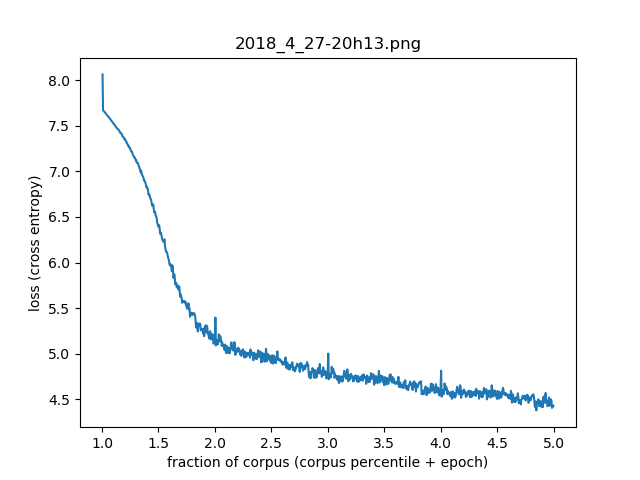
\includegraphics{parts/appendix/reports-gmsnn/docs_esteban-latex/test_reports/2018_4_27-20h13.png}
\caption{plot}
\end{figure}

\subsubsection{Details}

\begin{itemize}
\item
  log
  \href{https://gitlab.inria.fr/emarquer/awd-lstm-lm/blob/reimplement/logs/detrnn2018_4_27-14h11.log}{detrnn2018\_4\_27-14h11.log}
\item
  plot
  \href{https://gitlab.inria.fr/emarquer/awd-lstm-lm/blob/reimplement/plots/2018_4_27-20h13.png}{2018\_4\_27-16h42.png}
\end{itemize}

\subsection{Potential ameliorations \& next steps}

Next step is to test with more epochs, or test the growing model.

\end{report}
\begin{report}{Premier entraînement à 50 époques du modèle réimplémenté}\label{subsec:testreimp_3}
	% !TeX spellcheck = en_US
\section*{Test run of detrnn.py}

Test report

by E. Marquer, 2018/04/30, Synalp and Université de Lorraine

\subsection{Abstract}

Test to do a complete run on 50 epoch, with GPU, of the basic model of
DetRNN.

\subsection{Paradigm}

This test run of \emph{detrnn.py}, with INFO level log output, loss by
percentile and vbpc by epoch, will be executed with \emph{cuda}, for 50
epochs.

The test is done with branch
\href{https://gitlab.inria.fr/emarquer/awd-lstm-lm/tree/reimplement}{reimplement},
an allocated time of 76h, not interactive

Run time was estimated for 50 epochs according to the results for 4
epochs (see
\href{https://gitlab.inria.fr/emarquer/awd-lstm-lm/blob/master/docsEsteban/testReports/2018-04-27_test_run_detrnn.md}{2018-04-27\_test\_run\_detrnn.md}):

\begin{quote}
(5h 33min / 4 epoch) * 50 epoch = 4162.5min = 69h 22min 30s
\end{quote}

With a security margin of 10h, partially due to reduced batchsize, run
time is 80h.

\emph{/!\textbackslash{} Had to reduce batchsize down to 40 because of
memory errors /!\textbackslash{}}

\subsubsection{Node}

OAR\_JOB\_ID=155659 with GPU

Job start time: 2018-04-30 12:02:08

Estimated job stop time: 2018-05-03 16:02:08

Command used:
\lstinline!bash oarsub -q production -p "GPU <> 'NO'" -l "nodes=1,walltime=80:00:00" ~/awd-lstm-lm/rundet.sh!

\newpage
\subsection{Results}

Total run time for 50 epochs: with real stop time of 2018-05-02
17:16:56, the total run time of the training is aproximately 53h (2days
5h), corresponding to a little more than an hour per epoch.

BPC-wise, the DetRNN hardly goes under 2.7 even after 50 epoch, with a
change of 0.5 BPC in the last 30 epochs.

We can postulate that enven after 200 epoch, the DetRNN will not have a
BPC under 2.

\subsubsection{Plot}

\paragraph{BPC/fraction of corpus}

BPS per fraction of the corpus (an interval of 1 correspond a complete
corpus, or an epoch).

\begin{figure}[ht]
\centering
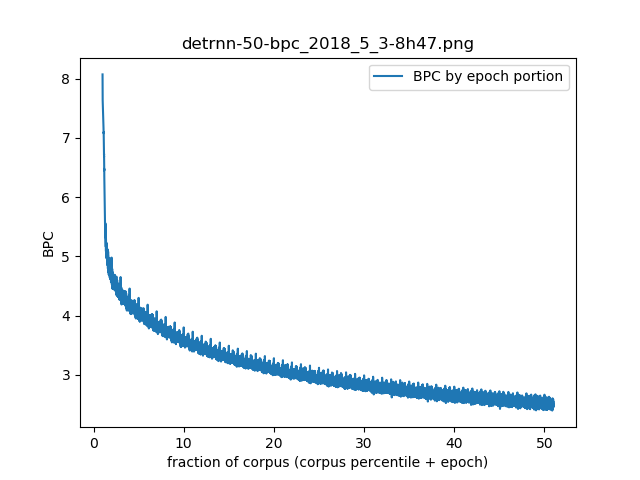
\includegraphics{parts/appendix/reports-gmsnn/docs_esteban-latex/test_reports/detrnn-50/detrnn-50-bpc_2018_5_3-8h47.png}
\caption{BPC}
\end{figure}

\newpage
\paragraph{ValBPC/epoch}

Mean BPC over the epoch, at the end of each epoch.

\begin{figure}[ht]
\centering
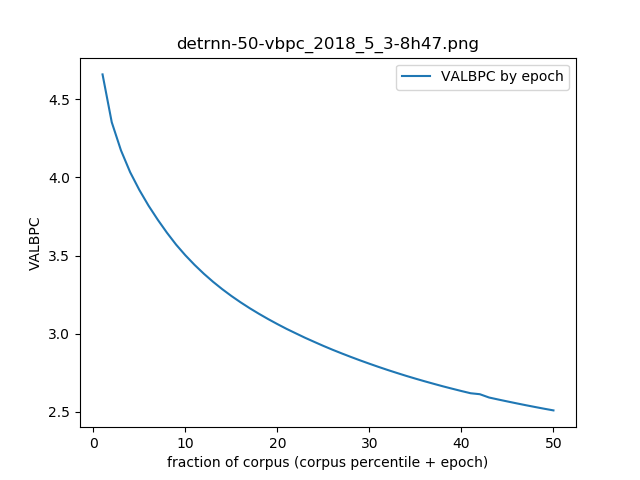
\includegraphics{parts/appendix/reports-gmsnn/docs_esteban-latex/test_reports/detrnn-50/detrnn-50-vbpc_2018_5_3-8h47.png}
\caption{ValBPC}
\end{figure}

\newpage
\paragraph{Loss}

Loss per fraction of the corpus (an interval of 1 correspond a complete
corpus, or an epoch).

\begin{figure}[ht]
\centering
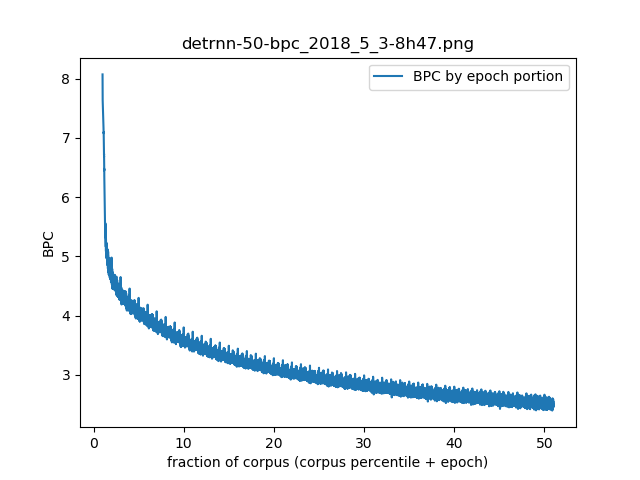
\includegraphics{parts/appendix/reports-gmsnn/docs_esteban-latex/test_reports/detrnn-50/detrnn-50-bpc_2018_5_3-8h47.png}
\caption{Loss}
\end{figure}

\subsubsection{Logs}

The log is available at 
\href{https://gitlab.inria.fr/emarquer/awd-lstm-lm/blob/reimplement/logs/detrnn-50_2018_4_30-12h2.log}{https://gitlab.inria.fr/emarquer/awd-lstm-lm/blob/reimplement/logs/detrnn-50\_2018\_4\_30-12h2.log}.

\subsection{Potential ameliorations \& next steps}

Next step is to test the growing model.

\end{report}
\begin{report}{Premier test du modèle multi-échelles}\label{subsec:testms}
	% !TeX spellcheck = en_US
\section*{Test run of detrnn.py}

Test report

by E. Marquer, 2018/05/03, Synalp and Université de Lorraine

\subsection{Abstract}

First performance test of the Test to do a run on 4 epochs, with GPU, of
the basic model of MSNN, with additive output strategy.

\subsection{Paradigm}

This test run of \emph{detrnn.py}, with DEBUG level log output, loss per
percentile and vbpc per epoch, that will be executed with \emph{cuda},
for 4 epochs.

The test is done with branch
\href{https://gitlab.inria.fr/emarquer/awd-lstm-lm/tree/growing}{growing},
an allocated time of 4h, not interactive.

Run time was estimated for 4 epochs according to a debug results for 0.2
epochs:

\begin{lstlisting}
(10min / 0.2 epoch) * 4 epoch = 200min = 3h 20min
\end{lstlisting}

With a security margin of 40min, run time is 4h.

\emph{/!\textbackslash{} Had to reduce batchsize down to 40 and halve
hidden size because of memoryerrors /!\textbackslash{}}

\newpage
\subsubsection{Hyperparameters}

\begin{longtable}[]{@{}ll@{}}
\hline
Hyperparameter & Value\tabularnewline
\hline
\endhead
nhidden & 920\tabularnewline
embedsize & 400\tabularnewline
bptt & 200\tabularnewline
batch\_size & 40\tabularnewline
eval\_batch\_size & 32\tabularnewline
lr & 0.001\tabularnewline
wdecay & 1.2e-06\tabularnewline
cuda\_on & True\tabularnewline
log\_interval & 20\tabularnewline
nepochs & 4\tabularnewline
max\_seqs & 15\tabularnewline
\hline
\end{longtable}

\subsubsection{Node}

OAR\_JOB\_ID=1558426 with GPU

Job start time: 2018-05-04 14:43:40

Estimated job stop time: 2018-05-04 18:43:40

Command used:

\begin{lstlisting}[language=bash]
oarsub -q production -p "GPU <> 'NO'" -l "nodes=1,walltime=04:00:00" ~/alt-repo/awd-lstm-lm/rundet.sh
\end{lstlisting}

Status verification loop:

\begin{lstlisting}[language=bash]
let x=0; while [ "true" ]; do echo "$x" $(oarstat -s -j 1558141); let ++x; sleep 120; done
\end{lstlisting}

\subsection{Results}

Total run time for 4 epochs: with real stop time of 2018-05-03 17:57:26,
the total run time of the training is aproximately 3h 13min,
corresponding to the predicted 50 min per epoch.

\newpage
\subsubsection{Comparative analysis}

With half the number of hidden parameters, and a yet unknown number of
layers, the basic MSNN has very similar results than the classical
DetRNN.

However, when analysing closely the learning speed, the MSNN seems to be
starting with a slower BPC decrease than the DetRNN, and it also seem to
be faster later on. Those variations are probably due to the number of
hidden layers.

\begin{figure}[h]
\centering
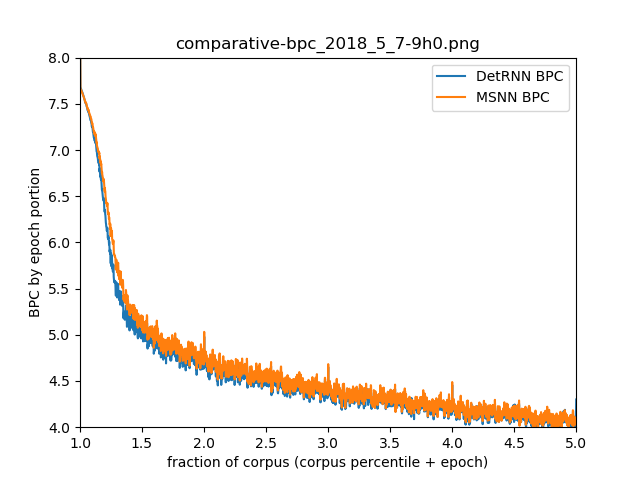
\includegraphics{parts/appendix/reports-gmsnn/docs_esteban-latex/test_reports/comparative-bpc-det-msnn_2018_5_7-9h0.png}
\caption{Comparative BPC}
\end{figure}

\subsubsection{Plot}

\paragraph{BPC/fraction of corpus}

BPS per fraction of the corpus (an interval of 1 correspond a complete
corpus, or an epoch).

\begin{figure}[h]
\centering
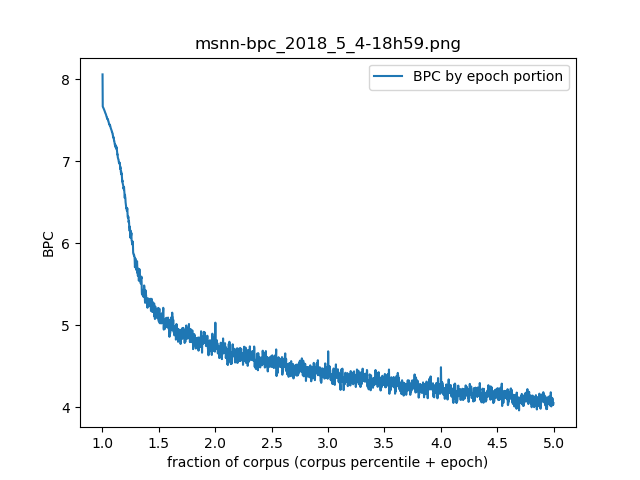
\includegraphics{parts/appendix/reports-gmsnn/docs_esteban-latex/test_reports/msnn-base/msnn-bpc_2018_5_4-18h59.png}
\caption{BPC}
\end{figure}

\paragraph{ValBPC/epoch}

Mean BPC over the epoch, at the end of each epoch.

\begin{figure}[h]
\centering
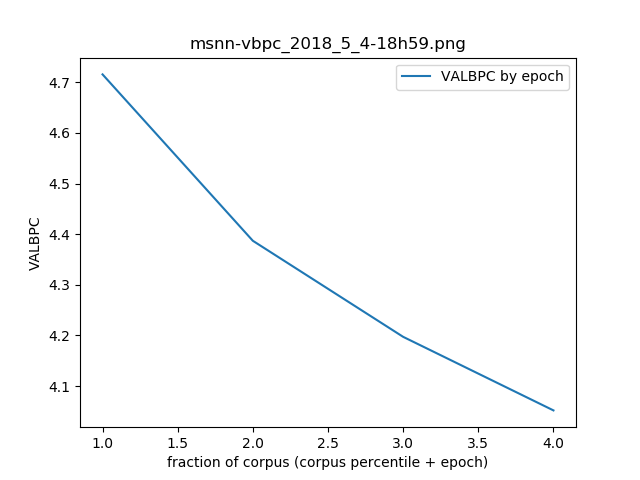
\includegraphics{parts/appendix/reports-gmsnn/docs_esteban-latex/test_reports/msnn-base/msnn-vbpc_2018_5_4-18h59.png}
\caption{ValBPC}
\end{figure}

\paragraph{Loss}

Loss per fraction of the corpus (an interval of 1 correspond a complete
corpus, or an epoch).

\begin{figure}[h]
\centering
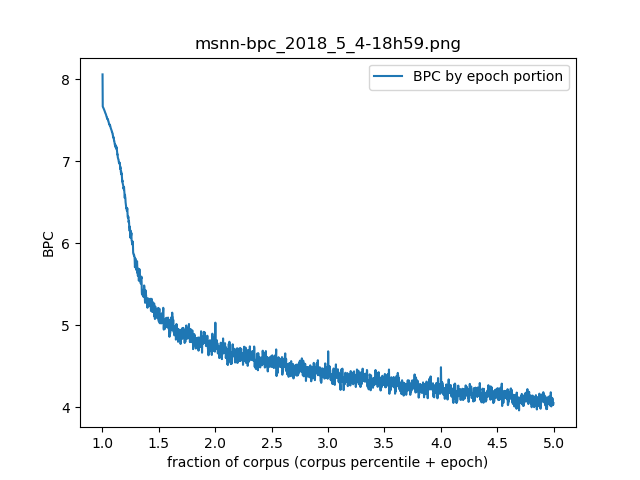
\includegraphics{parts/appendix/reports-gmsnn/docs_esteban-latex/test_reports/msnn-base/msnn-bpc_2018_5_4-18h59.png}
\caption{Loss}
\end{figure}

\subsubsection{Logs}

Reduced log is available at \href{msnn-base/msnn_2018_5_4-14h43.log}{msnn-base/msnn\_2018\_5\_4-14h43.log}.

\subsection{Potential ameliorations \& next steps}

A necessary amelioration is to add a way to track the number of layers.

As of now, the upper hidden layers participates in the output only when
updated. It is necessary to make them participate at every step.

The test process is not well defined: what to do when the eval batch is
dicontinuted from the training batch ? what if it is in the same corpus,
but not directly adjacent ? A possible yet hazardous solution would be
to evaluate a ``distance'' between the training and evaluation batches,
and reset the hidden states depending on that distance (a higher
distance would reset a higher number of layers).

Lastly, as the number of values to remember is increasing (bpc, loss,
layer number, \ldots{}) it would be interesting to improve the .plotdata
system.

Next step is to test the recurrently defined growing model.

\end{report}
\begin{report}{Comparaison des stratégies de fusion des résultats des différentes couches}\label{subsec:addcat}
	% !TeX spellcheck = en_US
\section*{Test run of detmsnn.py}

Test report

by E. Marquer, 2018/05/16, Synalp and Université de Lorraine

\subsection{Abstract}

Performance test of the `cat' (concatenated) output strategy compared to
the `add' strategy. Test to do a run on 4 epochs, with GPU, of the basic
model of MSNN, with concatenated output strategy.

\subsection{Paradigm}

This test run of \emph{detmsnn.py}, with INFO level log output, loss per
percentile and vbpc per epoch, is executed with \emph{cuda}, for 4
epochs.

The test is done with branch
\href{https://gitlab.inria.fr/emarquer/awd-lstm-lm/tree/growing}{growing},
an allocated time of 24h, not interactive

\textbf{/!\textbackslash{} Had to reduce evaluation courpus size down to
1/1000, to reduce computation time while keeping a big enough corpus to
compute BPC /!\textbackslash{}}

\newpage
\subsubsection{Hyperparameters}

\begin{longtable}[]{@{}ll@{}}
\hline
Hyperparameter & Value\tabularnewline
\hline
\endhead
nhidden & 920\tabularnewline
embedsize & 400\tabularnewline
bptt & 200\tabularnewline
batch\_size & 1\tabularnewline
eval\_batch\_size & 1\tabularnewline
lr & 0.001\tabularnewline
wdecay & 1.2e-06\tabularnewline
cuda\_on & True\tabularnewline
log\_interval & 100\tabularnewline
nepochs & 4\tabularnewline
max\_seqs & 5\tabularnewline
\hline
\end{longtable}

\subsubsection{Node}

OAR\_JOB\_ID=1563805 with GPU grimani-1

Job start time: 2018-05-16 08:53:20

Estimated job stop time: 2018-05-17 08:53:20

Command used:

\begin{lstlisting}[language=bash]
oarsub -q production -p "GPU <> 'NO'" -l "nodes=1,walltime=24:00:00" "bash runmsnn.sh"
\end{lstlisting}

Status verification loop:

\begin{lstlisting}[language=bash]
let x=0; while [ "true" ]; do echo "$x" $(oarstat -s -j 1563805); let ++x; sleep 120; done
\end{lstlisting}

\subsection{Results}

Total run time for 4 epochs: with real stop time of 08:53:28, the total
run time of the training is approximately 24h, with only 22\% of one
epoch done, and a final Validation BPC of 3.57.

Estimated run time for a full epoch: 24h / 22\% \textasciitilde{}=
109h/epoch. This corresponds to 436h for a 4 epoch run, and this is
critical.

The `cat' strategy is way more efficient in corpus consumption, even if
it is dramatically slower than the additive strategy.

\subsubsection{Comparative analysis}

The comparative plot shows that with the `cat' strategy, BPC diminution
is way faster than with the additive strategy. Computation-time wise, it
is obvious that the `cat' strategy is slower, with ??h/epoch, than the
`add' strategy, with 50min/epoch. This difference is too large to be due
to the device alone.

\begin{figure}[h]
\centering
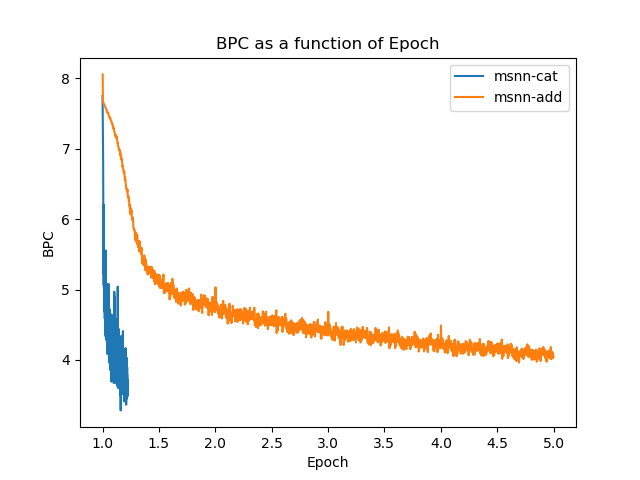
\includegraphics{parts/appendix/reports-gmsnn/docs_esteban-latex/test_reports/comparative-bpc-msnn-det-msnn-cat.png}
\caption{Comparative BPC}
\end{figure}

\subsubsection{Plot}

\paragraph{BPC/fraction of corpus}

BPC: BPC per fraction of the corpus (an interval of 1 correspond a
complete corpus, or an epoch).

Validation BPC: BPC per fraction of the corpus, on the validation
corpus.

Layers: Number of layers per fraction of the corpus.
\begin{figure}[h]
	\centering
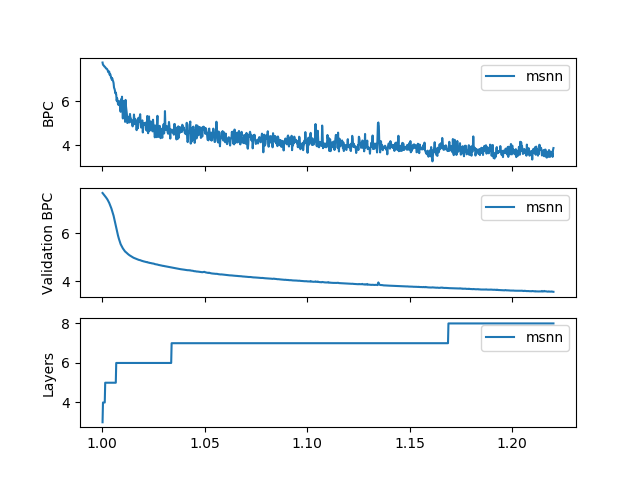
\includegraphics{parts/appendix/reports-gmsnn/docs_esteban-latex/test_reports/msnn-4/2018_05_17-13h49.png}
\caption{Comparative BPC}
\end{figure}

\newpage
\subsection{Potential ameliorations \& next steps}

Next step is to try to reduce run time.

\end{report}
\begin{report}{Test des effets du changement de taille des paquets (\foreign{batch})}\label{subsec:batch_1}
	% !TeX spellcheck = en_US
\section*{Test run of detmsnn.py}

Test report

by E. Marquer, 2018/05/16, Synalp and Université de Lorraine

\subsection{Abstract}

Performance test of batch size variation without deeper . Test to do a
run on 4 epochs, with GPU, of the basic model of MSNN, with concatenated
output strategy.

\subsection{Paradigm}

This test run of \emph{detmsnn.py}, with INFO level log output, loss per
percentile and vbpc per epoch, is executed with \emph{cuda}, for 4
epochs.

The test is done with branch
\href{https://gitlab.inria.fr/emarquer/awd-lstm-lm/tree/growing}{growing},
an allocated time of 24h, not interactive

\textbf{/!\textbackslash{} Had to reduce evaluation corpus size down to
1/1000, to reduce computation time while keeping a big enough corpus to
compute BPC /!\textbackslash{}}

\subsubsection{Hyperparameters}

\begin{longtable}[]{@{}ll@{}}
\hline
Hyperparameter & Value\tabularnewline
\hline
\endhead
nhidden & 920\tabularnewline
embedsize & 400\tabularnewline
bptt & 200\tabularnewline
batch\_size & 16\tabularnewline
lr & 0.001\tabularnewline
wdecay & 1.2e-06\tabularnewline
cuda\_on & True\tabularnewline
log\_interval & 100\tabularnewline
save\_interval & 100\tabularnewline
nepochs & 4\tabularnewline
max\_seqs & 5\tabularnewline
\hline
\end{longtable}

\subsubsection{Node}

OAR\_JOB\_ID=1567202 with GPU grimani-1

Planed job start time: 2018-05-19 02:41:08 Job start time: 2018-05-19
02:41:08

Estimated job stop time: 2018-05-22 14:41:08

Command used:

\begin{lstlisting}[language=bash]
oarsub -q production -p "GPU <> 'NO'" -l "nodes=1,walltime=84:00:00" "bash runmsnn.sh"
\end{lstlisting}

Status verification loop:

\begin{lstlisting}[language=bash]
let x=0; while [ "true" ]; do echo "$x" $(oarstat -s -j 1567202); let ++x; sleep 120; done
\end{lstlisting}

\subsection{Results}

Total run time for 4 epochs: with real stop time of ?, the total run
time of the training is approximately ?h, with only, and a final
Validation BPC of 3.57.

\subsubsection{Comparative analysis}

\textbf{NO PLOT HERE}

\subsubsection{Plot}

\paragraph{BPC/fraction of corpus}

BPC: BPC per fraction of the corpus (an interval of 1 correspond a
complete corpus, or an epoch).

Validation BPC: BPC per fraction of the corpus, on the validation
corpus.

Layers: Number of layers per fraction of the corpus. 

\textbf{NO PLOT HERE}

\subsection{Potential ameliorations \& next steps}

Next step is to continue run time reduction.

\end{report}


\begin{report}{Entraînement sur le corpus complet avec beaucoup de temps alloué}\label{subsec:long_train}
	% !TeX spellcheck = en_US
\section*{Long-run of RNN-MSNN}

Test report

by E. Marquer, 2018/05/29, Synalp and Université de Lorraine

\subsection{Abstract}

The run was done on the reduced enwik8 corpus.

The test is composed of 4 successive runs:
\begin{itemize}
	\item 1 run of 2h on grimani-4;
	\item 2 runs of 12h, both on grimani-1;
	\item 1 run of 50h on grele-11;
\end{itemize}

End causes are as follow: 
\begin{itemize}
	\item Run 1: out of time (2h);
	\item Run 2: out of time (12h);
	\item Run 3: end of epoch crash (7h30);
	\item Run 4: end of epoch crash (19h15);
\end{itemize}

Mean time for an epoch is about 19h 15min (on the reduced version of the
corpus). Two epochs were completed.

\subsection{Results}

Each run crashed between epochs, so a bit of patching had to be made on
top of fixing the bug.

\subsubsection{Memory}

Both RAM and video RAM are still subject to a constant leak in memory.
But even if it does not show on the plots (scale is too small), logs
confirm that there is no leak during validation.

\begin{figure}[H]
\centering
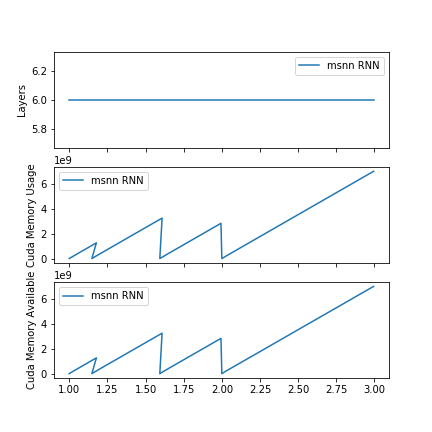
\includegraphics{parts/appendix/reports-gmsnn/docs_esteban-latex/test_reports/2018-06-11/memory.png}
\caption{Memory usage}
\end{figure}

\begin{figure}[H]
\centering
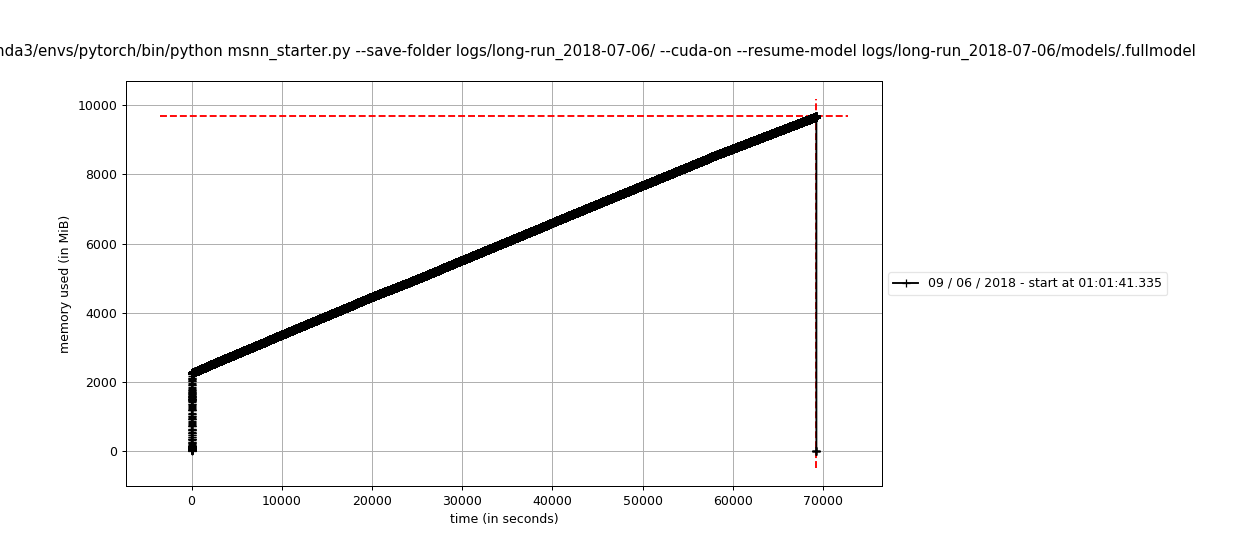
\includegraphics[width=\textwidth]{parts/appendix/reports-gmsnn/docs_esteban-latex/test_reports/2018-06-11/RAM_restart-2.png}
\caption{RAM third run}
\end{figure}

An other noticeable property is that ``Run Time'', corresponding to the
time to train over \emph{log\_interval} sequences, is mostly
proportional to CUDA memory usage. The source of the cuda memory leak is
probably the same as what makes training slower.

\begin{figure}[H]
\centering
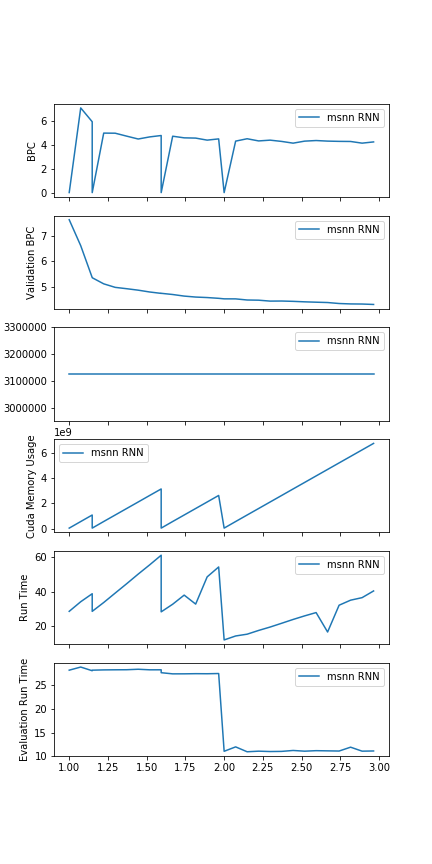
\includegraphics[height=.8\textheight]{parts/appendix/reports-gmsnn/docs_esteban-latex/test_reports/2018-06-11/frac.png}
\caption{Memory and computation time}
\end{figure}

\newpage
\subsubsection{BPC / Validation BPC}

BPC and Validation BPC

\begin{figure}[H]
\centering
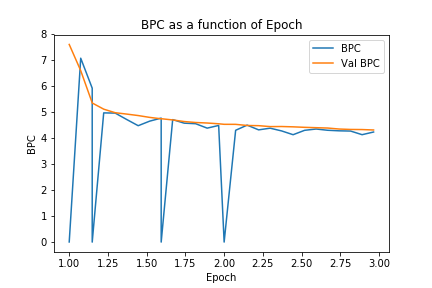
\includegraphics[width=\textwidth]{parts/appendix/reports-gmsnn/docs_esteban-latex/test_reports/2018-06-11/frac_val_bpc.png}
\caption{BPC}
\end{figure}


\newpage
\subsubsection{Job restart}\label{job-restart}

When resuming a job, CUDA memory is entirely freed. Same thing can be
said about RAM.

\begin{figure}[H]
\centering
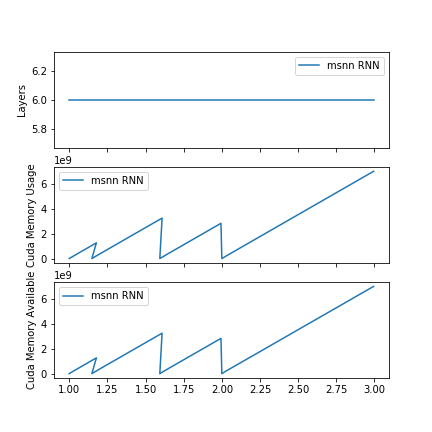
\includegraphics[width=\textwidth]{parts/appendix/reports-gmsnn/docs_esteban-latex/test_reports/2018-06-11/memory.png}
\caption{Memory usage}
\end{figure}

\begin{figure}[H]
\centering
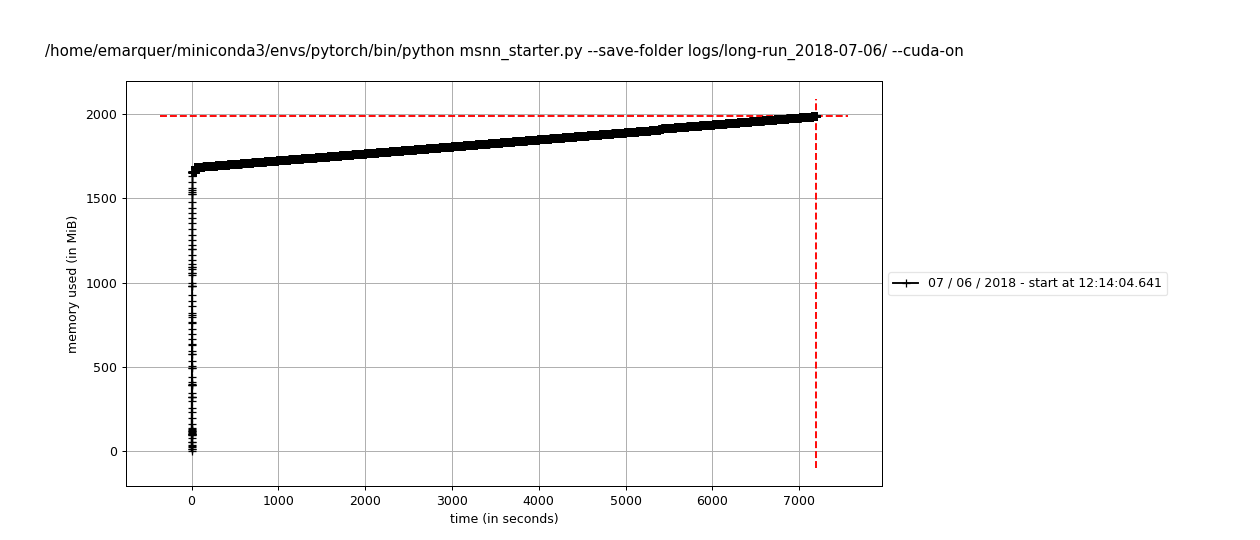
\includegraphics[width=\textwidth]{parts/appendix/reports-gmsnn/docs_esteban-latex/test_reports/2018-06-11/RAM.png}
\caption{RAM first run}
\end{figure}

\begin{figure}[H]
\centering
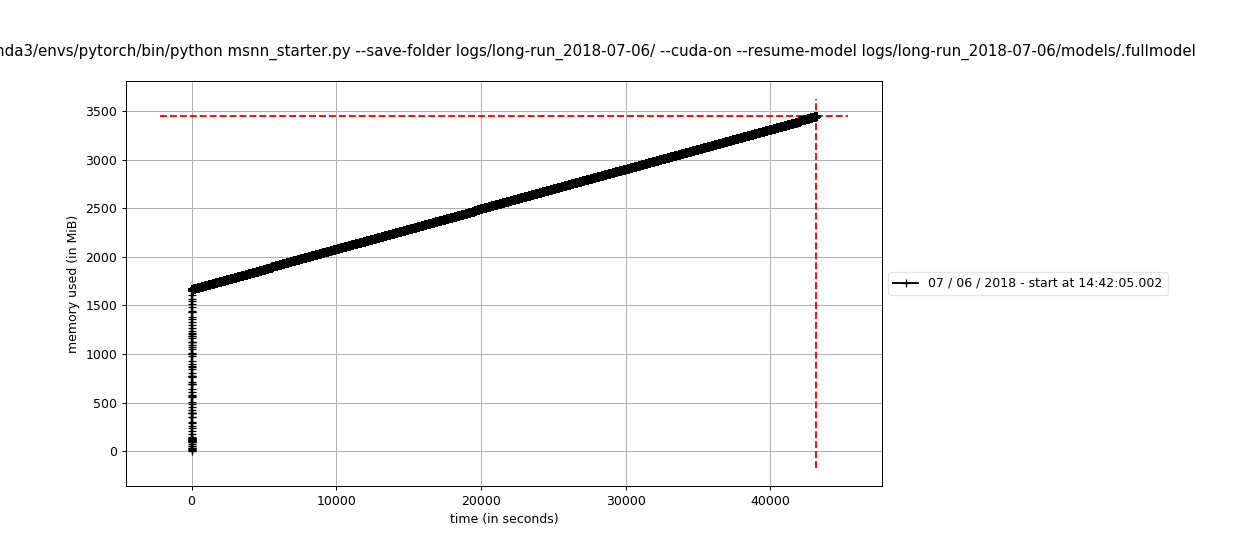
\includegraphics[width=\textwidth]{parts/appendix/reports-gmsnn/docs_esteban-latex/test_reports/2018-06-11/RAM_restart-1.png}
\caption{RAM second run}
\end{figure}

\begin{figure}[H]
\centering
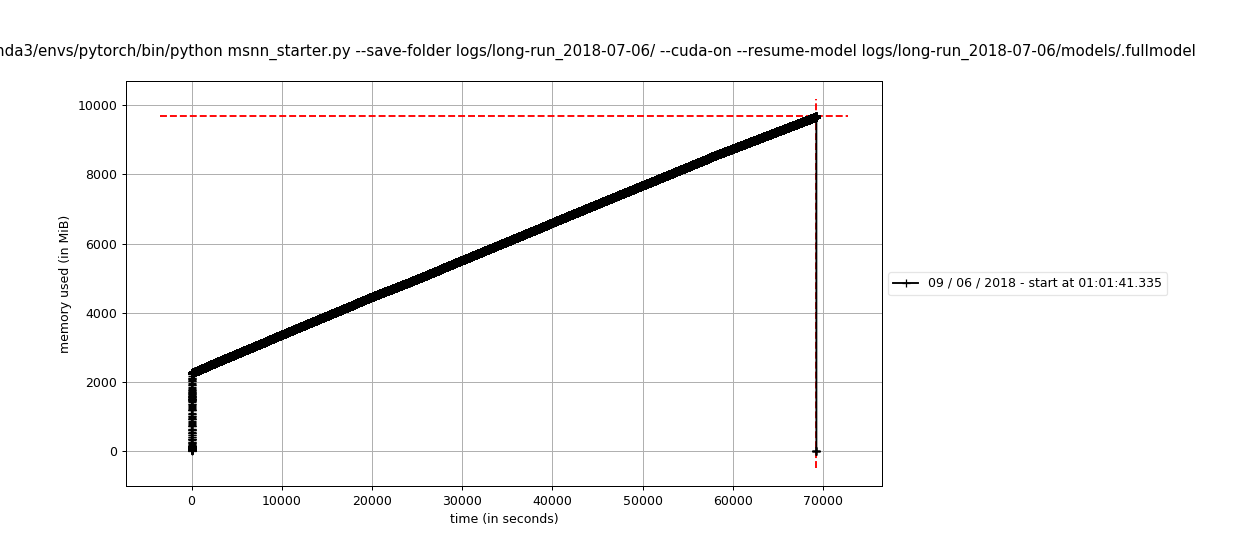
\includegraphics[width=\textwidth]{parts/appendix/reports-gmsnn/docs_esteban-latex/test_reports/2018-06-11/RAM_restart-2.png}
\caption{RAM third run}
\end{figure}

Memory is freed each time the job is restarted, meaning either a part of
the necessary is discarded, or unnecessary data is kept in memory. As in
CUDAles tests a memory maximum was reached, CUDA seems to be the source
of the leak (data copies not removed, \ldots{}).

\subsection{Next steps}

Debug end of epoch bug. Try to patch memory leak. Continue training.

\end{report}
\begin{report}{Changement de stratégie de gestion d'historique}\label{subsec:change_history}
	\section*{Change history}

Analysis report

by E. Marquer, 2018/06/12, Synalp and Université de Lorraine

\subsection{Abstract}

As computation graph has been confirmed to exist/be considered only in
the last history, keeping an explicit history is no longer necessary.
Worst, it may hinder garbage collection, by keeping references to
Tensors that are completely useless.

A new model of history has been made to keep only a reference to the
last hidden state. This new model will be referred as ``last'', and the
old one keeping an explicit history as ``classical''.

\subsection{Tests}

Multiple tests were done on the new ``enwik8mini'' corpus of 100,000 characters:
\begin{itemize}
\item ``last'' a test run on 2 epochs with 1 batches of ``last'' history
\item ``last b2'' a test run on 10 epochs with 2 batches of ``last'' history
\item ``last b2 10epoch'' a test run on 10 epochs with 2 batches of ``last'' history
\item ``classical'' a test run on 2 epochs with 1 batches of ``classical'' history
\end{itemize}

\subsubsection{Results (1 epoch)}

The results are over 1 epoch, with values from the start of the first
and the second epoch. As ``last b2 10epoch'' and ``last b2'' have the
same set of parameters, they coincides.

\begin{figure}[h]
\centering
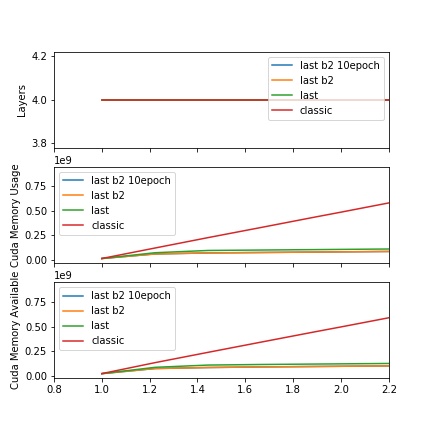
\includegraphics{parts/appendix/reports-gmsnn/docs_esteban-latex/test_reports/2018-06-12/history_memory_1e.png}
\caption{Memory 1 epoch}
\end{figure}

\begin{figure}[h]
\centering
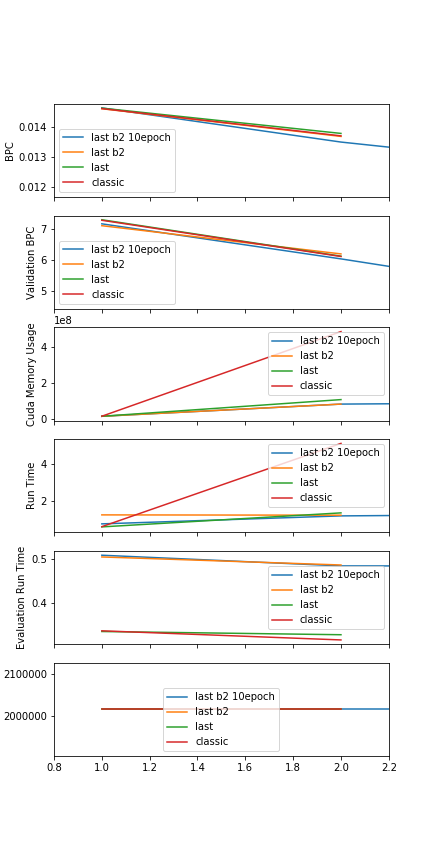
\includegraphics{parts/appendix/reports-gmsnn/docs_esteban-latex/test_reports/2018-06-12/history_frac_1e.png}
\caption{All info 1 epoch}
\end{figure}

\subsubsection{Results (full)}

\begin{figure}[h]
\centering
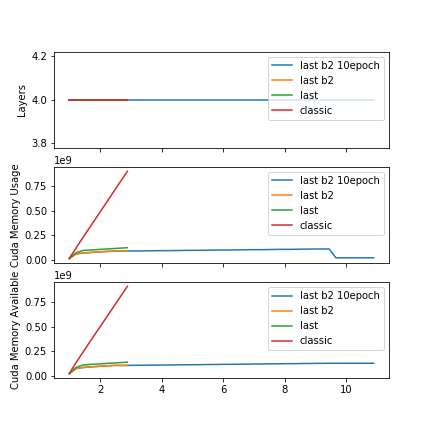
\includegraphics{parts/appendix/reports-gmsnn/docs_esteban-latex/test_reports/2018-06-12/history_memory.png}
\caption{Memory}
\end{figure}

\begin{figure}[h]
\centering
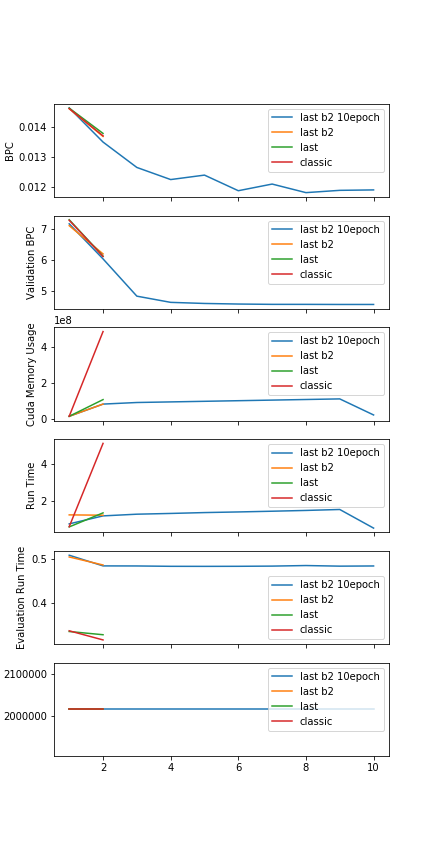
\includegraphics{parts/appendix/reports-gmsnn/docs_esteban-latex/test_reports/2018-06-12/history_frac.png}
\caption{All info}
\end{figure}

\paragraph{\texorpdfstring{Ram consumption for ``last b2 10epoch''}{Ram consumption for last b2 10epoch}}

\begin{figure}[h]
\centering
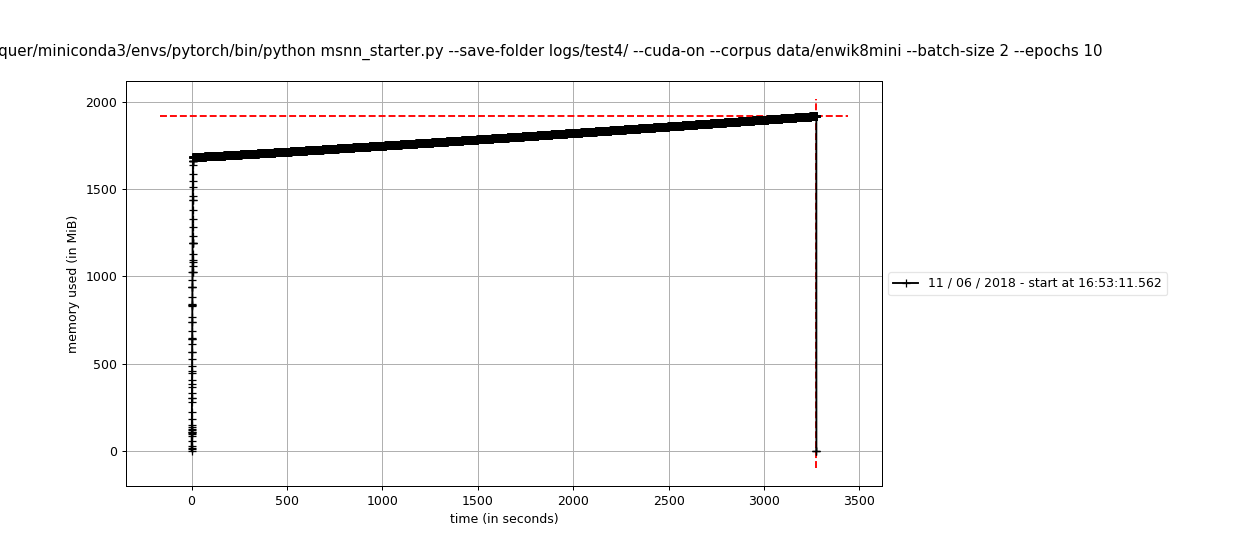
\includegraphics{parts/appendix/reports-gmsnn/docs_esteban-latex/test_reports/2018-06-12/history_RAM.png}
\caption{RAM 10 epoch}
\end{figure}

\subsection{Conclusion}

\subsubsection{Memory leak}

The leak in CUDA memory has reduced drastically.

It seems there is still a leak, this leak is not present when CUDA is
not used. This leak is present in both RAM and graphical RAM, but the
remaining leak in graphical RAM is not a concern anymore, with only a
dozen MiB over 1,000,000 characters (10 epochs * 100,000 characters).
However, the leak in RAM has not reduced, and even if it is not a
problem thanks to the available RAM in the cluster, it would be
preferable to identify the source of the leak.

\subsubsection{Run (training) time}

Additionally, the correlation of CUDA memory usage and and training run
time is kept, so the small remaining CUDA leak is probably linked to the
computation graph. With CUDA memory usage drastically reduced, run time
has been reduced too.

Currently, training over 100,000 characters (with 2 batches) only takes
5 minutes.

\subsubsection{Performances}

No conclusion can be drawn on learning performances, due to the size of
the learning corpus. Even though, it is encouraging that even with a
small corpus 10 epochs are not enough to have over-fitting (at least
with 2 batches).

\subsection{Next steps}

\begin{enumerate}
\def\labelenumi{\arabic{enumi}.}
\item
  long training over the ``enwik8reduced'' or the ``enwik8'' corpus;
\item
  fix (or at least identify) RAM leak
\end{enumerate}

\end{report}
\begin{report}{Test de l'implémentation des \foreign{batchs}}\label{subsec:test_batch}\label{subsec:batch_2}
	\section*{Long-run of RNN-MSNN}

Test report

by E. Marquer, 2018/06/13 Synalp and Université de Lorraine

\subsection{Abstract}

The test is composed of 2 successive runs:
\begin{itemize}
\item id 1582586: batch-size 1, bptt 200 on grele-4;
\item id 1582587: batch-size 2, bptt 100 on grimani-6.
\end{itemize}

Run time is about 10h in each case, corresponding to 2h30 for an epoch.
In both case corpus batches rotation over epochs was disabled.

\subsubsection{Shared parameters}

\begin{longtable}[]{@{}ll@{}}
\hline
parameter & value\tabularnewline
\hline
\endhead
corpus & enwik8reduced\tabularnewline
history\_strategy & layer-constant-length\tabularnewline
max\_history & 25\tabularnewline
bptt & \emph{variable}\tabularnewline
batch\_size & \emph{variable}\tabularnewline
epochs & 4\tabularnewline
lr & 1e-3\tabularnewline
weight\_decay & 1.2e-6\tabularnewline
epochs & 4\tabularnewline
valid\_len & 500,000\tabularnewline
log\_interval & 500\tabularnewline
save\_interval & 500\tabularnewline
memory\_interval & 100\tabularnewline
hidden\_size & 460\tabularnewline
embed\_size & 400\tabularnewline
growth\_factor & 5\tabularnewline
rnn\_type & RNN\tabularnewline
reset\_hidden & False\tabularnewline
reset\_growth & True\tabularnewline
cuda\_on & True\tabularnewline
\hline
\end{longtable}

\subsection{Results}

At the end of each epoch, we see a spike in BPC, due to the first
evaluation of the epoch. As corpus rotation is disabled, it is not
surprising that with two batches over-fitting appears.

Moreover, we can note that run time is constant and memory usage tend to
a constant value (1.6 GiB), with no difference between 1 and 2 batches.
Note: the product \lstinline!bptt * batch_size! is equal for 1 and 2
batches, so this result is the one predicted by the equations.

\begin{figure}[h]
\centering
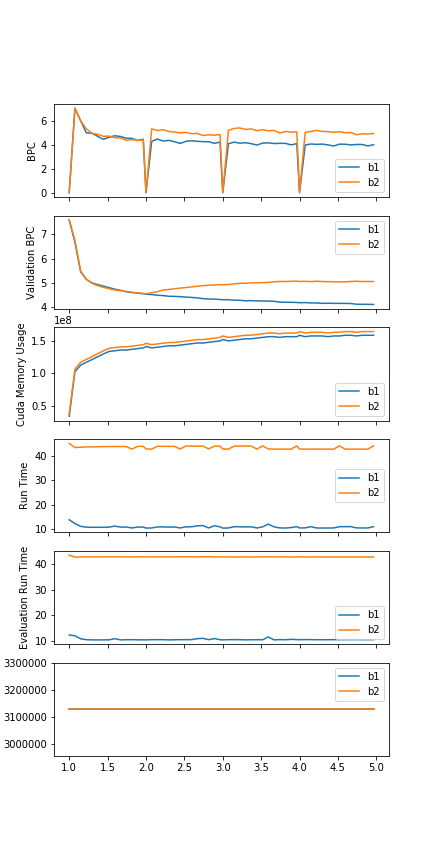
\includegraphics{parts/appendix/reports-gmsnn/docs_esteban-latex/test_reports/2018-06-13/batch_1_2_frac.png}
\caption{RAM third run}
\end{figure}

\begin{figure}[h]
\centering
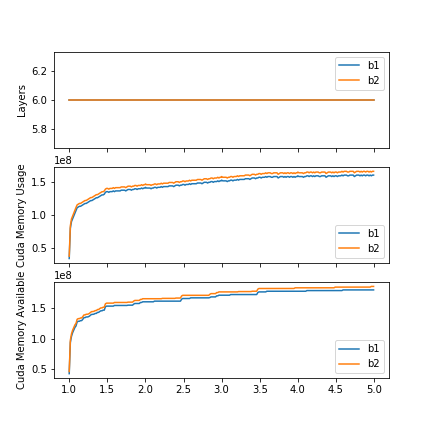
\includegraphics{parts/appendix/reports-gmsnn/docs_esteban-latex/test_reports/2018-06-13/batch_1_2_memory.png}
\caption{Memory usage}
\end{figure}

\subsection{Next steps}

\begin{itemize}
\item
  batches:

  \begin{enumerate}
  \def\labelenumi{\arabic{enumi}.}
  \item
    Implement corpus rotation
  \item
    See if corpus rotation solves over-fitting
  \item
    Compare run time on comparable machines
  \end{enumerate}
\item
  long run:

  \begin{enumerate}
  \def\labelenumi{\arabic{enumi}.}
  \item
    Continue batch 1 for more epochs
  \item
    See when over-fitting appears
  \end{enumerate}
\end{itemize}

\end{report}
\begin{report}{Test des performances des \foreign{batchs}}\label{subsec:test_batch_perf}\label{subsec:batch_3}
	\section{Run on the same node of RNN-MSNN with different batch
size}\label{run-on-the-same-node-of-rnn-msnn-with-different-batch-size}

Test report

by E. Marquer, 2018/06/15 Synalp and Université de Lorraine

\subsection{Abstract}\label{abstract}

The test is composed of 2 runs: - id 1583339: batch-size 1, bptt 200 on
grele-2 - id 1583336: batch-size 2, bptt 100 on grele-1

Run time per epoch varies from 28 to 20 min for a single batch and from
20 to 11 min for two batches.

\subsubsection{Shared parameters}\label{shared-parameters}

\begin{longtable}[]{@{}ll@{}}
\toprule
parameter & value\tabularnewline
\midrule
\endhead
corpus & enwik8reduced\tabularnewline
history\_strategy & layer-constant-length\tabularnewline
max\_history & 25\tabularnewline
bptt & \emph{variable}\tabularnewline
batch\_size & \emph{variable}\tabularnewline
epochs & 4\tabularnewline
lr & 1e-3\tabularnewline
weight\_decay & 1.2e-6\tabularnewline
epochs & 4\tabularnewline
valid\_len & 500,000\tabularnewline
log\_interval & 500\tabularnewline
save\_interval & 500\tabularnewline
memory\_interval & 100\tabularnewline
hidden\_size & 460\tabularnewline
embed\_size & 400\tabularnewline
growth\_factor & 5\tabularnewline
rnn\_type & RNN\tabularnewline
reset\_hidden & False\tabularnewline
reset\_growth & True\tabularnewline
cuda\_on & True\tabularnewline
\bottomrule
\end{longtable}

\subsection{Results}\label{results}

At the end of each epoch, we see a spike in BPC, due to the first
evaluation of the epoch (BPC is reinitialised to 0, causing a spike).
With 2 btches, BPC is also more stable.

As of now, run time is computed after running validation, so training
time is \lstinline!real_training_time = run_time - validation_time!. But
validation time increase with the number of batches as the number of
characters seen increase (the whole validation corpus is used for each
batch, so the number of characters seen during validation is
\lstinline!validation_corpus_len * batches!). That explains that the
evaluation time for a batch is lower than for 2 batches.

By removing evaluation time, we can obtain a reasonable and coherent
(with regard to epoch run time) estimation of training time over a
sequence.

\subsubsection{Epoch run time:}\label{epoch-run-time}

\begin{longtable}[]{@{}lll@{}}
\toprule
Epoch & Run time b=1 & Run time b=2\tabularnewline
\midrule
\endhead
1 & 28 min & 20 min\tabularnewline
2 & 23 min & 17 min\tabularnewline
3 & 22 min & 14 min\tabularnewline
4 & 20 min & 11 min\tabularnewline
\bottomrule
\end{longtable}

There is a notable decrease in epoch run time (time necessary to run
over an epoch), of about 10 min over the 4 epochs, with both runs.

Possible causes for the decrease of run time: - part of the graph is
already computed, and this part is skipped; - corpus data is already
loaded in cuda memory.

Both of them are highly unlikely to cause such a decrease. A more
precise training time storage may provide an explanation.

\subsubsection{Plots}\label{plots}

\begin{figure}
\centering
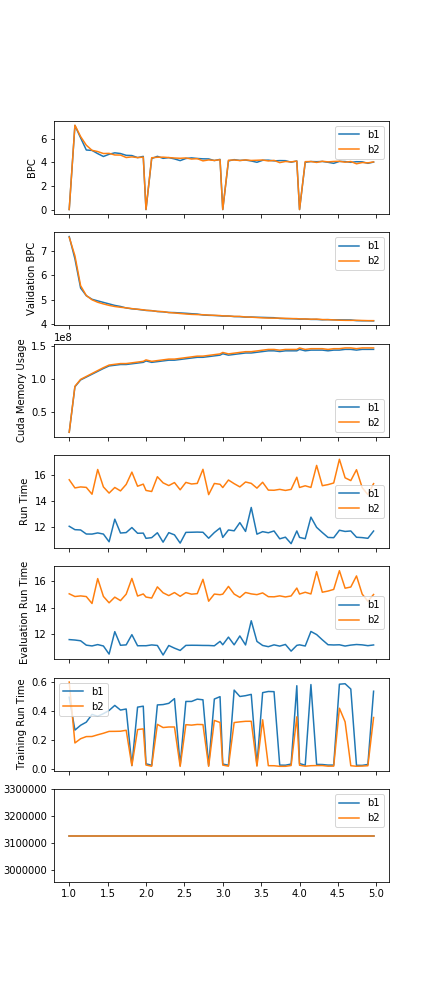
\includegraphics{2018_06_15_frac.png}
\caption{Full data}
\end{figure}

\begin{figure}
\centering
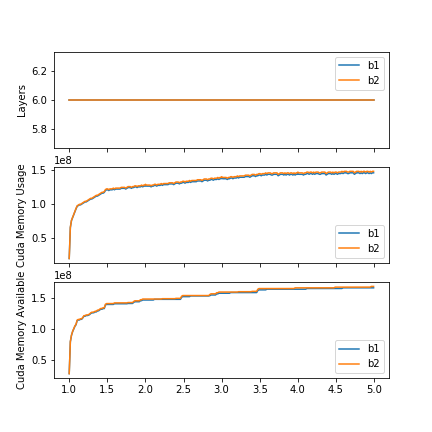
\includegraphics{2018_06_15_memory.png}
\caption{Memory usage}
\end{figure}

\subsection{Next steps}\label{next-steps}

\begin{itemize}
\tightlist
\item
  Data

  \begin{itemize}
  \tightlist
  \item
    Implement more precise time data saving (epoch run time and training
    run time)
  \end{itemize}
\item
  Runs (objective: 100 epochs)

  \begin{itemize}
  \tightlist
  \item
    Continue running batches 1 and 2
  \item
    Try with higher number of batches
  \end{itemize}
\item
  {[}Optional{]} Other experimental branch

  \begin{enumerate}
  \def\labelenumi{\arabic{enumi}.}
  \tightlist
  \item
    Implement prepared attention module in every layer
  \item
    Analyse results
  \item
    Patch probable memory leaks
  \end{enumerate}
\end{itemize}

\end{report}
\begin{report}{Test des performances des \foreign{batchs} sur 50 époques}\label{subsec:test_batch_perf_}\label{subsec:batch_4}
	\section{Run over more than 50 epochs with varied batch
size}\label{run-over-more-than-50-epochs-with-varied-batch-size}

Test report

by E. Marquer, 2018/06/19 Synalp and Université de Lorraine

\subsection{Abstract}\label{abstract}

The test is composed of 4 runs on grele, with: - bptt 200, batch-size 1
- bptt 100, batch-size 2 - bptt 50, batch-size 4 - bptt 25, batch-size 8

Run has been interrupted by an overflow of disk space due to the
detailed logs; next runs will used reduced logs.

Run time per epoch varies from 30 to 7 min.

\subsubsection{Shared parameters}\label{shared-parameters}

\begin{longtable}[]{@{}ll@{}}
\toprule
parameter & value\tabularnewline
\midrule
\endhead
corpus & enwik8reduced\tabularnewline
history\_strategy & layer-constant-length\tabularnewline
max\_history & 25\tabularnewline
bptt & \emph{variable}\tabularnewline
batch\_size & \emph{variable}\tabularnewline
epochs & 4\tabularnewline
lr & 1e-3\tabularnewline
weight\_decay & 1.2e-6\tabularnewline
epochs & 4\tabularnewline
valid\_len & 500,000\tabularnewline
log\_interval & 500\tabularnewline
save\_interval & 500\tabularnewline
memory\_interval & 100\tabularnewline
hidden\_size & 460\tabularnewline
embed\_size & 400\tabularnewline
growth\_factor & 5\tabularnewline
rnn\_type & RNN\tabularnewline
reset\_hidden & False\tabularnewline
reset\_growth & True\tabularnewline
cuda\_on & True\tabularnewline
\bottomrule
\end{longtable}

\subsection{Results}\label{results}

At the end of each epoch, we see a spike in BPC, due to the first
evaluation of the epoch (BPC is reinitialised to 0, causing a spike).
With any number of batch, while keeping the
\lstinline!bptt * batch_size! ratio, BPC and Validation BPC do not vary.

Even with 200 epochs, with batch size of 1, there is no trace of
over-fitting.

\subsubsection{Epoch run time:}\label{epoch-run-time}

\begin{longtable}[]{@{}lllll@{}}
\toprule
Epoch & Run time b=1 & Run time b=2 & Run time b=4 & Run time
b=8\tabularnewline
\midrule
\endhead
1 & 30 min & 21 min & 18 min & 19 min\tabularnewline
10 & 21 min & 14 min & 14 min & 17 min\tabularnewline
\textgreater{}15 & 7 min & 7 min & 8 min & 11 min\tabularnewline
\bottomrule
\end{longtable}

\begin{longtable}[]{@{}lll@{}}
\toprule
Epoch 1 & Epoch 10 & Epoch 15\tabularnewline
\midrule
\endhead
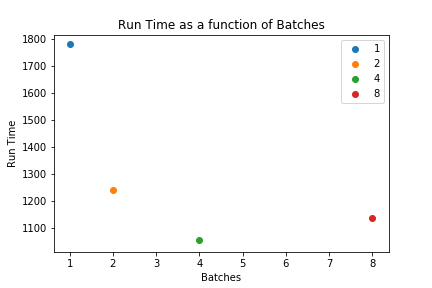
\includegraphics{b1a8_batch_epoch_1.png} &
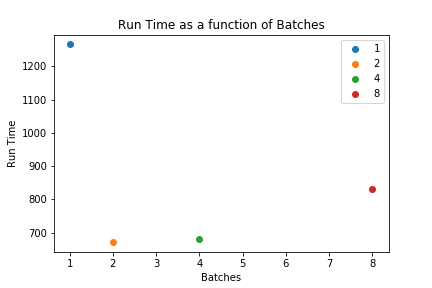
\includegraphics{b1a8_batch_epoch_10.png} &
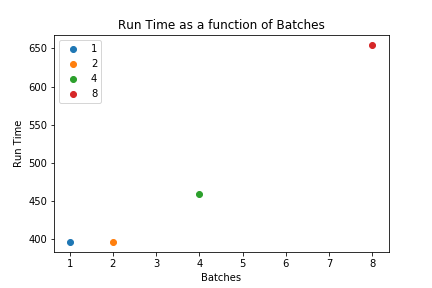
\includegraphics{b1a8_batch_epoch_15.png}\tabularnewline
\bottomrule
\end{longtable}

Run time can be split over two set of epochs: before, and after the 15th
epoch. Before the 15th epoch, run is faster with more batches, with the
exception of batch-size 8, which is slower than batch-size 2 and 4.
After the 15th epoch, run is slower with more batches.

To optimize run time, it is necessary to balance run time before 15
epochs. If a high number of batches is planed (\textgreater{}50),
between 2 and 4 batches are preferable, because the run time after epoch
15 has a lot of impact on global run time; however, if only a few epochs
are planed (\textless{}20), a high number of batches is preferable, as
run time before epoch 15 is the most important.

With current corpus, 2, 3 or 4 batches are the most interesting setup.

Decrease in run time is most probably due to the history of the upper
layers, that needs multiple epochs to fill.

\subsubsection{Plots}\label{plots}

\paragraph{BPC}\label{bpc}

\begin{figure}
\centering
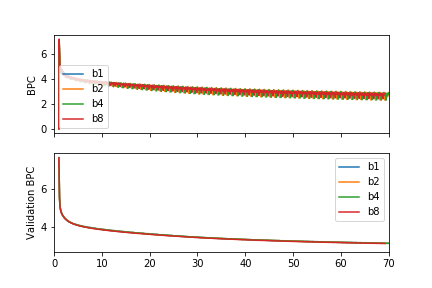
\includegraphics{b1a8_frac.png}
\caption{Full data}
\end{figure}

\begin{figure}
\centering
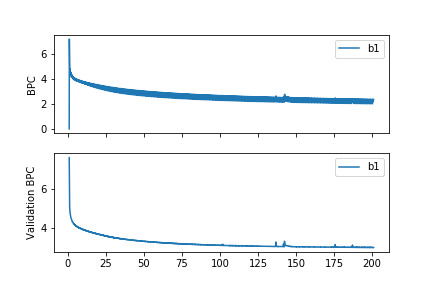
\includegraphics{b1a8_200.png}
\caption{Full data}
\end{figure}

\paragraph{Memory}\label{memory}

\begin{figure}
\centering
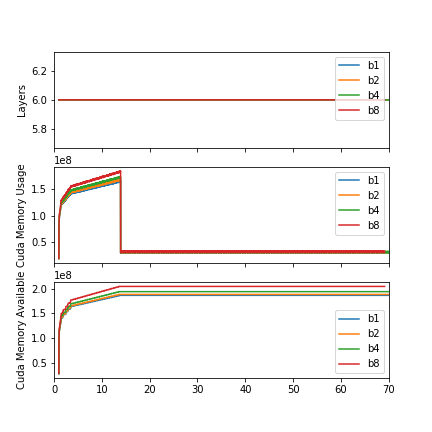
\includegraphics{b1a8_memory.png}
\caption{Full data}
\end{figure}

\paragraph{Run time (in seconds)}\label{run-time-in-seconds}

\begin{figure}
\centering
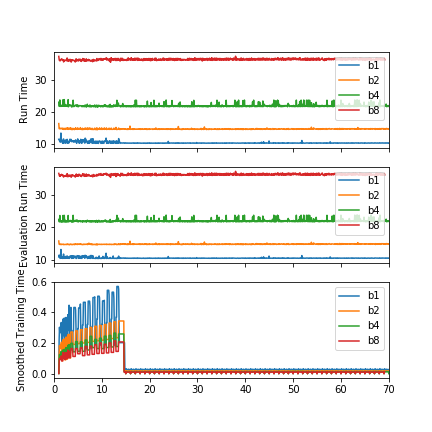
\includegraphics{b1a8_time.png}
\caption{Run time}
\end{figure}

\subparagraph{Epoch run time}\label{epoch-run-time-1}

\begin{figure}
\centering
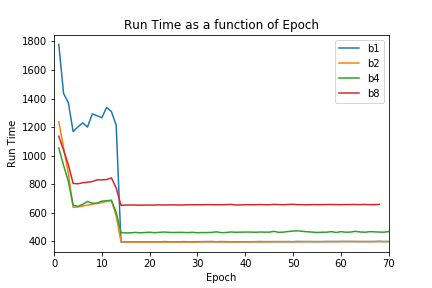
\includegraphics{b1a8_epoch.png}
\caption{Epoch run time}
\end{figure}

\subsection{Next steps}\label{next-steps}

\begin{itemize}
\tightlist
\item
  Independent impact of batch number and sequence length:

  \begin{itemize}
  \tightlist
  \item
    Run with fixed batch number and varying sequence length
  \item
    Run with fixed sequence length and varying batch number
  \end{itemize}
\item
  Impact of corpus length on optimal number of batch and sequences:

  \begin{itemize}
  \tightlist
  \item
    Run with varying sequence length and varying batch number over the
    full length corpus
  \end{itemize}
\item
  Number of parameters:

  \begin{itemize}
  \tightlist
  \item
    Increase the hidden layer size
  \end{itemize}
\item
  {[}Future{]} Transmission rate impact:

  \begin{itemize}
  \tightlist
  \item
    Compare optimal values of parameters, and BPC reached with varying
    transmission rate
  \end{itemize}
\end{itemize}

\end{report}
\begin{report}{Test des performances des différentes améliorations}\label{subsec:test_perf}
	\section{Run over more than 50 epochs with varied batch
size}\label{run-over-more-than-50-epochs-with-varied-batch-size}

Test report

by E. Marquer, 2018/06/19 Synalp and Université de Lorraine

\subsection{Abstract}\label{abstract}

The test runs are for two parallel experiments: - test which of 2 and 3
batches are the most interesting - test the impact of layer by layer
training (with an intuitive algorithm developed out of work-time)

The test is composed of 4 runs on grele, with: - bptt 200/2, batch-size
2 - bptt 200/3, batch-size 3 - bptt 200/2, batch-size 2, layer by layer
training, - bptt 200/2, batch-size 2, layer by layer training, 20 epochs
of individual training for each layer, 10 epochs of common fine-tuning
for already trained layers (see below the explanation of this algorithm)

\subsubsection{Shared parameters}\label{shared-parameters}

\begin{longtable}[]{@{}ll@{}}
\toprule
parameter & value\tabularnewline
\midrule
\endhead
corpus & enwik8reduced\tabularnewline
history\_strategy & last\tabularnewline
max\_history & 25\tabularnewline
lr & 1e-3\tabularnewline
weight\_decay & 1.2e-6\tabularnewline
epochs & 1500\tabularnewline
valid\_len & 500,000\tabularnewline
log\_interval & 500\tabularnewline
save\_interval & 500\tabularnewline
memory\_interval & 100\tabularnewline
hidden\_size & 460\tabularnewline
embed\_size & 400\tabularnewline
growth\_factor & 5\tabularnewline
rnn\_type & RNN\tabularnewline
reset\_hidden & False\tabularnewline
reset\_growth & True\tabularnewline
cuda\_on & True\tabularnewline
\bottomrule
\end{longtable}

\subsubsection{Model keys and
specificities}\label{model-keys-and-specificities}

When noting is specified, all models have:

\begin{itemize}
\tightlist
\item
  2 batches, and a sequence length of 200/2
\item
  1 RNN layer per MSNN layer
\end{itemize}

\begin{longtable}[]{@{}ll@{}}
\toprule
\begin{minipage}[b]{0.08\columnwidth}\raggedright\strut
Model\strut
\end{minipage} & \begin{minipage}[b]{0.86\columnwidth}\raggedright\strut
Specificity\strut
\end{minipage}\tabularnewline
\midrule
\endhead
\begin{minipage}[t]{0.08\columnwidth}\raggedright\strut
b2\strut
\end{minipage} & \begin{minipage}[t]{0.86\columnwidth}\raggedright\strut
classical model, comparison basis\strut
\end{minipage}\tabularnewline
\begin{minipage}[t]{0.08\columnwidth}\raggedright\strut
b3\strut
\end{minipage} & \begin{minipage}[t]{0.86\columnwidth}\raggedright\strut
3 batches, sequence length of 200/3\strut
\end{minipage}\tabularnewline
\begin{minipage}[t]{0.08\columnwidth}\raggedright\strut
s\strut
\end{minipage} & \begin{minipage}[t]{0.86\columnwidth}\raggedright\strut
``scheduled(10,10)'': use layer by layer training; 10 epochs for
individual training, 10 epochs for intermediary fine-tuning\strut
\end{minipage}\tabularnewline
\begin{minipage}[t]{0.08\columnwidth}\raggedright\strut
s-a20-l10\strut
\end{minipage} & \begin{minipage}[t]{0.86\columnwidth}\raggedright\strut
``scheduled(20,10)'': use layer by layer training; 20 epochs for
individual training, 10 epochs for intermediary fine-tuning\strut
\end{minipage}\tabularnewline
\begin{minipage}[t]{0.08\columnwidth}\raggedright\strut
l2\strut
\end{minipage} & \begin{minipage}[t]{0.86\columnwidth}\raggedright\strut
2 RNN layer per MSNN layer\strut
\end{minipage}\tabularnewline
\begin{minipage}[t]{0.08\columnwidth}\raggedright\strut
l3\strut
\end{minipage} & \begin{minipage}[t]{0.86\columnwidth}\raggedright\strut
3 RNN layer per MSNN layer\strut
\end{minipage}\tabularnewline
\begin{minipage}[t]{0.08\columnwidth}\raggedright\strut
s\_l3\_a\strut
\end{minipage} & \begin{minipage}[t]{0.86\columnwidth}\raggedright\strut
3 RNN layer per MSNN layer, ``scheduled(10,10)'' (see model ``s''),
attentive intermediary input\strut
\end{minipage}\tabularnewline
\bottomrule
\end{longtable}

\subsubsection{Series}\label{series}

\begin{longtable}[]{@{}llll@{}}
\toprule
\begin{minipage}[b]{0.04\columnwidth}\raggedright\strut
Series\strut
\end{minipage} & \begin{minipage}[b]{0.08\columnwidth}\raggedright\strut
Model\strut
\end{minipage} & \begin{minipage}[b]{0.30\columnwidth}\raggedright\strut
Respective name of models on plots\strut
\end{minipage} & \begin{minipage}[b]{0.46\columnwidth}\raggedright\strut
Objective\strut
\end{minipage}\tabularnewline
\midrule
\endhead
\begin{minipage}[t]{0.04\columnwidth}\raggedright\strut
b2\_b3\strut
\end{minipage} & \begin{minipage}[t]{0.08\columnwidth}\raggedright\strut
b2, b3\strut
\end{minipage} & \begin{minipage}[t]{0.30\columnwidth}\raggedright\strut
``b2'', ``b3''\strut
\end{minipage} & \begin{minipage}[t]{0.46\columnwidth}\raggedright\strut
Compare training with 2 and 3 batches\strut
\end{minipage}\tabularnewline
\begin{minipage}[t]{0.04\columnwidth}\raggedright\strut
l\strut
\end{minipage} & \begin{minipage}[t]{0.08\columnwidth}\raggedright\strut
b2, l2, l3\strut
\end{minipage} & \begin{minipage}[t]{0.30\columnwidth}\raggedright\strut
``1 RNN layer'', ``2 RNN layers'', ``3 RNN layers''\strut
\end{minipage} & \begin{minipage}[t]{0.46\columnwidth}\raggedright\strut
See impact of number of RNN layers\strut
\end{minipage}\tabularnewline
\begin{minipage}[t]{0.04\columnwidth}\raggedright\strut
lbl\strut
\end{minipage} & \begin{minipage}[t]{0.08\columnwidth}\raggedright\strut
b2, s, s-a20-l10\strut
\end{minipage} & \begin{minipage}[t]{0.30\columnwidth}\raggedright\strut
``Classical'', ``Layer by layer (10, 10)'', ``Layer by layer (20,
10)''\strut
\end{minipage} & \begin{minipage}[t]{0.46\columnwidth}\raggedright\strut
See impact of layer by layer training\strut
\end{minipage}\tabularnewline
\begin{minipage}[t]{0.04\columnwidth}\raggedright\strut
sum\strut
\end{minipage} & \begin{minipage}[t]{0.08\columnwidth}\raggedright\strut
b2, s\_l3\_a\strut
\end{minipage} & \begin{minipage}[t]{0.30\columnwidth}\raggedright\strut
``Classical'', ``3 RNN layers, LbL, attentive''\strut
\end{minipage} & \begin{minipage}[t]{0.46\columnwidth}\raggedright\strut
Check if layer by layer training, atentive model, and multi-RNN-layered
architectures are compatibles\strut
\end{minipage}\tabularnewline
\bottomrule
\end{longtable}

\subsection{Results}\label{results}

\begin{longtable}[]{@{}llllll@{}}
\toprule
Series & Time & Time to run an epoch & Memory & BPC & Full length
BPC\tabularnewline
\midrule
\endhead
b2\_b3 & 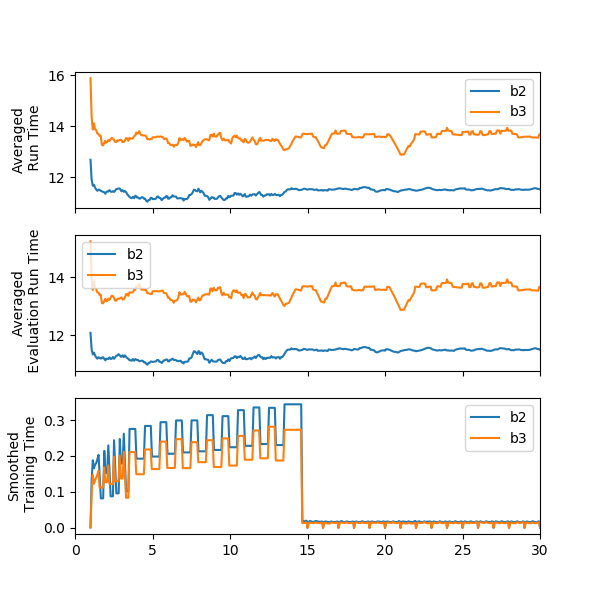
\includegraphics{b2_b3_time.png} &
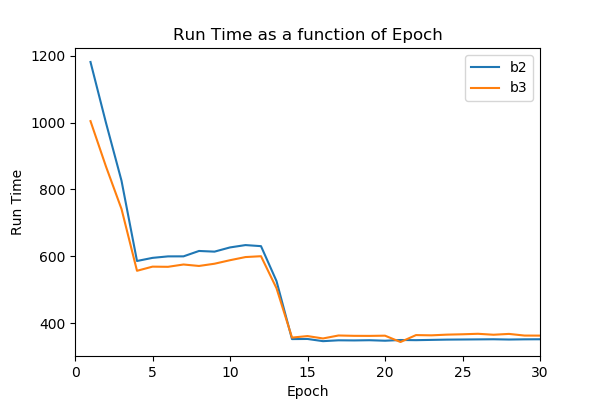
\includegraphics{b2_b3_epoch.png} & 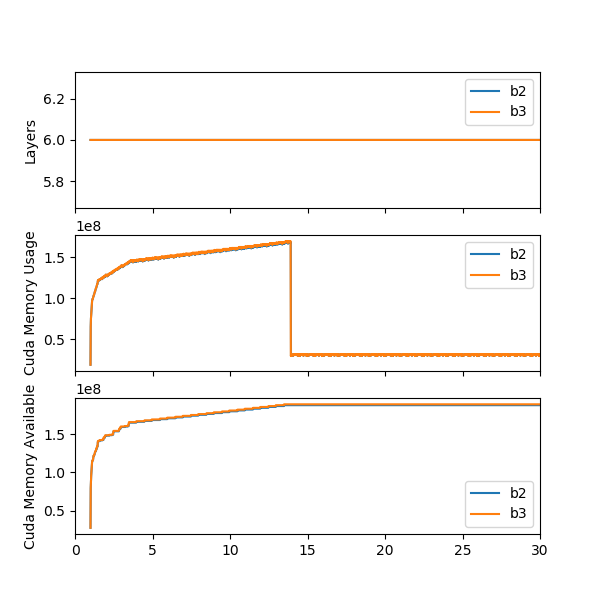
\includegraphics{b2_b3_memory.png} &
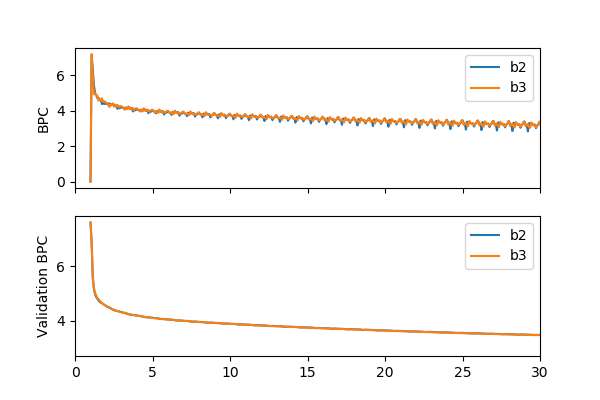
\includegraphics{b2_b3_frac.png} &
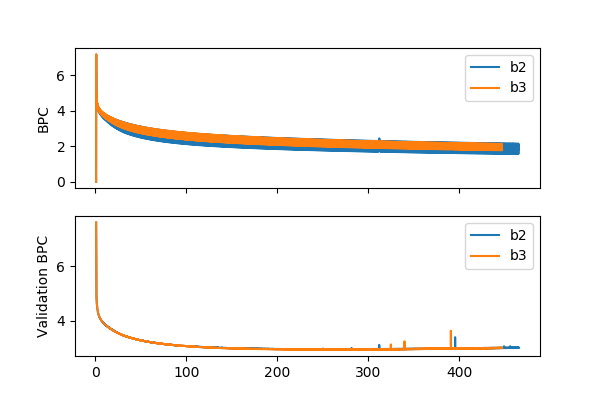
\includegraphics{b2_b3_frac_full.png}\tabularnewline
l & 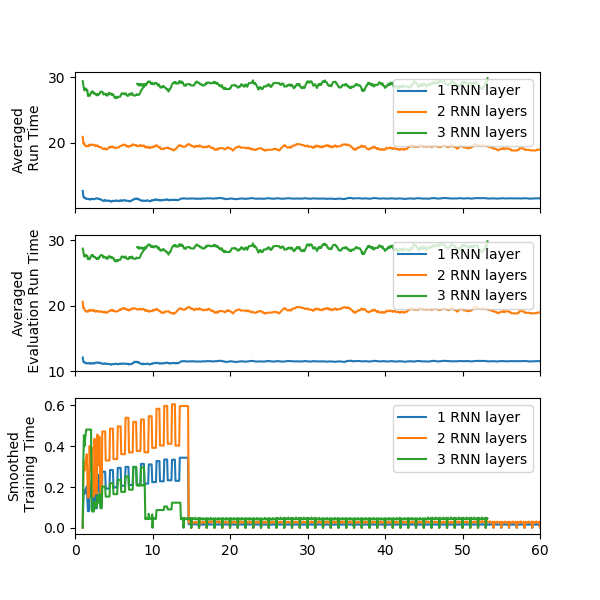
\includegraphics{l_time.png} & 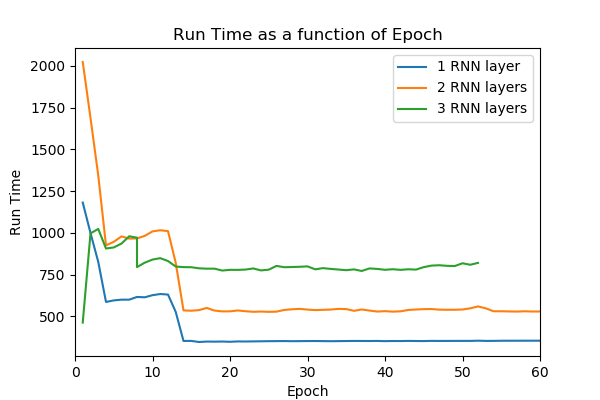
\includegraphics{l_epoch.png} &
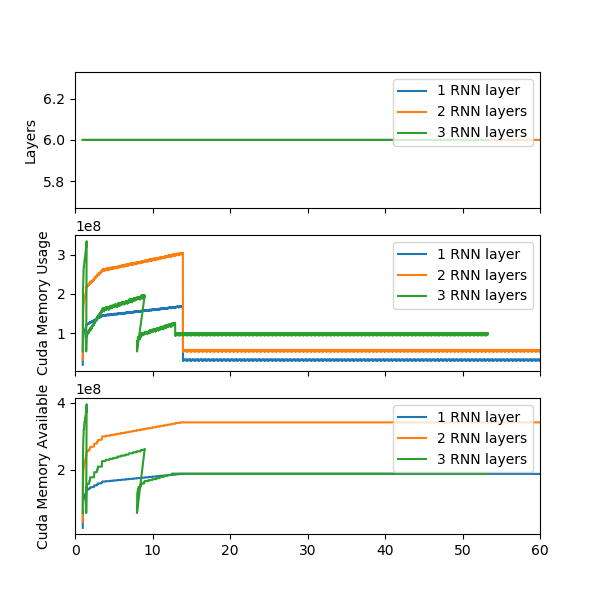
\includegraphics{l_memory.png} & 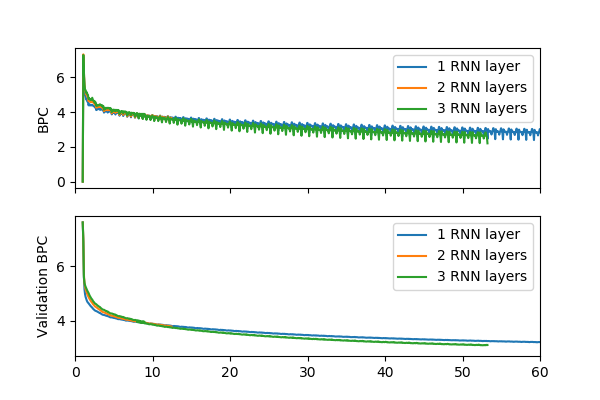
\includegraphics{l_frac.png} &
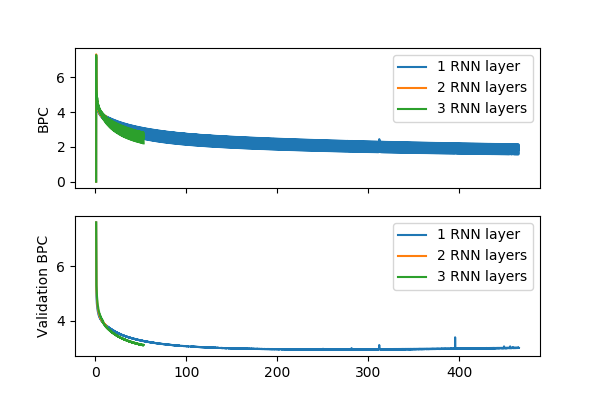
\includegraphics{l_frac_full.png}\tabularnewline
lbl & 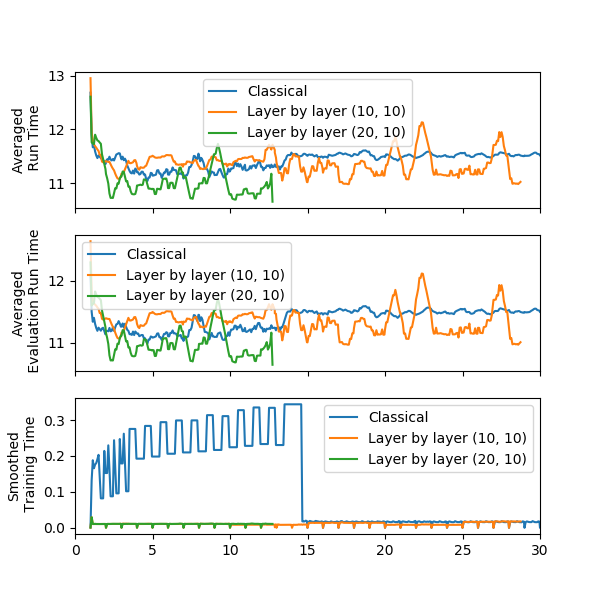
\includegraphics{lbl_time.png} & 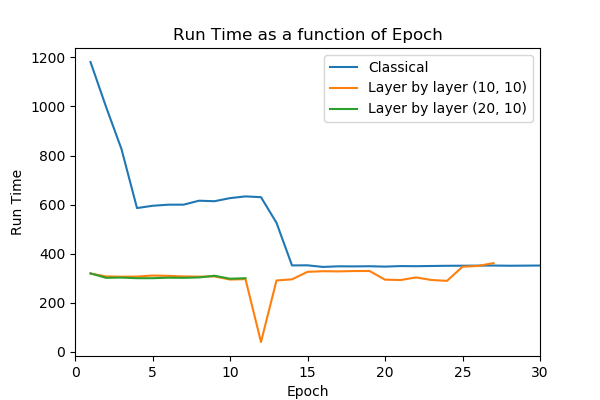
\includegraphics{lbl_epoch.png} &
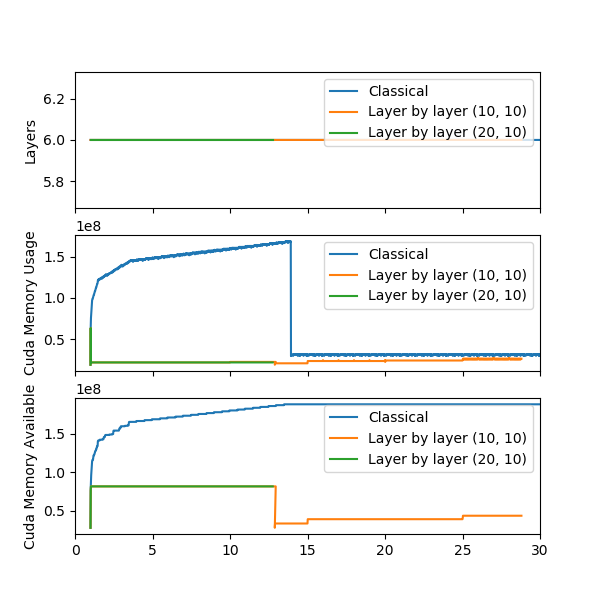
\includegraphics{lbl_memory.png} & 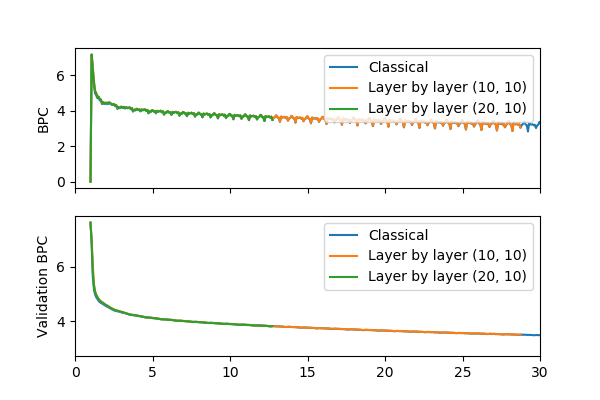
\includegraphics{lbl_frac.png} &
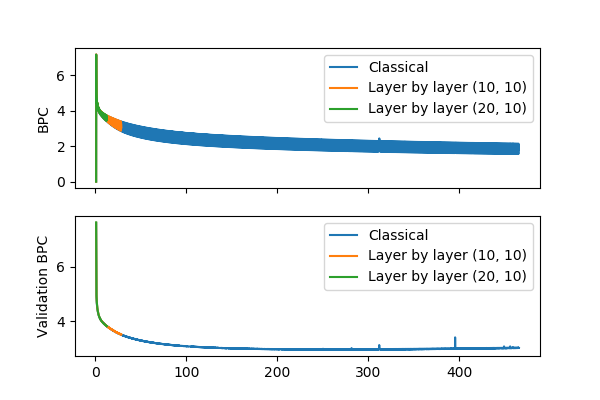
\includegraphics{lbl_frac_full.png}\tabularnewline
sum & \includegraphics{sum_time.png} & \includegraphics{sum_epoch.png} &
\includegraphics{sum_memory.png} & \includegraphics{sum_frac.png} &
\includegraphics{sum_frac_full.png}\tabularnewline
\bottomrule
\end{longtable}

Plots will be referred to with : (Ex: ``l:Memory'')

\subsubsection{Time necessary to reach indicated validation
BPC}\label{time-necessary-to-reach-indicated-validation-bpc}

\begin{longtable}[]{@{}lrrr@{}}
\toprule
Model & 5 BPC & 4 BPC & 3 BPC\tabularnewline
\midrule
\endhead
b2 & 0H 19M 41S & 1H 19M 47S & 15H 13M 7S\tabularnewline
b3 & 0H 16M 44S & 1H 11M 48S & 15H 3M 22S\tabularnewline
s & 0H 5M 19S & 0H 30M 59S &\tabularnewline
s-a20-l10 & 0H 5M 19S & 0H 30M 26S &\tabularnewline
l2 & 0H 33M 43S & 2H 27M 51S &\tabularnewline
l3 & \sout{0H 7M 41S} & \sout{2H 13M 2S} &\tabularnewline
s\_l3\_a & 0H 16M 7S & &\tabularnewline
\bottomrule
\end{longtable}

Empty fields are where network has not reached BPC yet \sout{Crossed
out} fields are where data has been corrupted (because of an
interruption in training)

\subsubsection{Epochs necessary to reach indicated validation
BPC}\label{epochs-necessary-to-reach-indicated-validation-bpc}

\begin{longtable}[]{@{}llll@{}}
\toprule
Model & 5 BPC & 4 BPC & 3 BPC\tabularnewline
\midrule
\endhead
b2 & 0.296 & 6.000 & 141.4\tabularnewline
b3 & 0.367 & 5.954 & 136.4\tabularnewline
s & 0.371 & 6.000 &\tabularnewline
s-a20-l10 & 0.371 & 6.000 &\tabularnewline
l2 & 0.593 & 6.519 &\tabularnewline
l3 & 0.816 & 7.296 &\tabularnewline
s\_l3\_a & 1.148 & &\tabularnewline
\bottomrule
\end{longtable}

Empty fields are where network has not reached BPC yet

\subsection{Analysis}\label{analysis}

\subsubsection{\texorpdfstring{Run time and memory on ``l'' series
(l:memory, l:time, and l:time to run an
epoch)}{Run time and memory on l series (l:memory, l:time, and l:time to run an epoch)}}\label{run-time-and-memory-on-l-series-lmemory-ltime-and-ltime-to-run-an-epoch}

Training of ``l3'' model was interrupted 2 times before the 15th epoch,
each time cleaning the memory, inducing training time reduction and
epoch time reduction (due to the correlation of memory usage and
training time).

\subsubsection{\texorpdfstring{Run time and memory on ``lbl'' series
(lbl:memory, lbl:time, and lbl:time to run an
epoch)}{Run time and memory on lbl series (lbl:memory, lbl:time, and lbl:time to run an epoch)}}\label{run-time-and-memory-on-lbl-series-lblmemory-lbltime-and-lbltime-to-run-an-epoch}

The specificity of layer by layer training are a lead to the cause of
the collapse of memory usage and run time during the 15th epoch.

During layer by layer training, memory usage is kept constant over the
first 15 epochs, whereas with classical training, memory usage increases
during ths period.

Layer by layer training reduces simultaneous graph accumulation over the
different epochs by training a layer at a time. It possibly reduces SGD
inertia too.

\subsubsection{Performance of layer by layer
training}\label{performance-of-layer-by-layer-training}

No notable variation on BPC. For run time and memory, see above.

\subsubsection{Performance of multi-RNN-layered
architecture}\label{performance-of-multi-rnn-layered-architecture}

A slight improvement of BPC can be seen with 3 layers (sadly, BPC data
for 2 layers is corrupted). Computation-time is proportional to the
number of layers (time data for 3 layers is unusable).

\subsubsection{Performance of 3 batches compared to 2
batches}\label{performance-of-3-batches-compared-to-2-batches}

2 and 3 batches have an almost identical performance (time-wise,
BPC-wise and memory-wise), except 3 batches seem to get less dispersed
BPC.

\subsubsection{Results of long training with 2 and 3 batches
(b2\_b3:full length
bpc)}\label{results-of-long-training-with-2-and-3-batches-b2_b3full-length-bpc}

The plot ``b2\_b3:full length bpc'' shows that after 200 epochs,
validation BPC stagnates. After 300 epochs, validation BPC begins to
increase very slowly, those are the first signs of over-fitting. These
observations were cross-checked with the raw data.

\subsubsection{Note on attention module}\label{note-on-attention-module}

A model with the attention module was tested for 5 hours, and did not
reach a full epoch. It can be deemed that without a training algorithm
like layer by layer training, using attention is not viable.

\end{report}





%\input{parts/appendix/reports-gmsnn/docs_esteban-latex/}